\documentclass[11pt]{article}

    \usepackage[breakable]{tcolorbox}
    \usepackage{parskip} % Stop auto-indenting (to mimic markdown behaviour)
    \usepackage{lmodern}
    \usepackage{iftex}
    \ifPDFTeX
    	\usepackage[T1]{fontenc}
    	\usepackage{mathpazo}
    \else
    	\usepackage{fontspec}
    \fi

    % Basic figure setup, for now with no caption control since it's done
    % automatically by Pandoc (which extracts ![](path) syntax from Markdown).
    \usepackage{graphicx}
    % Maintain compatibility with old templates. Remove in nbconvert 6.0
    \let\Oldincludegraphics\includegraphics
    % Ensure that by default, figures have no caption (until we provide a
    % proper Figure object with a Caption API and a way to capture that
    % in the conversion process - todo).
    \usepackage{caption}
    \DeclareCaptionFormat{nocaption}{}
    \captionsetup{format=nocaption,aboveskip=0pt,belowskip=0pt}

    \usepackage{float}
    \floatplacement{figure}{H} % forces figures to be placed at the correct location
    \usepackage{xcolor} % Allow colors to be defined
    \usepackage{enumerate} % Needed for markdown enumerations to work
    \usepackage{geometry} % Used to adjust the document margins
    \usepackage{amsmath} % Equations
    \usepackage{amssymb} % Equations
    \usepackage{textcomp} % defines textquotesingle
    % Hack from http://tex.stackexchange.com/a/47451/13684:
    \AtBeginDocument{%
        \def\PYZsq{\textquotesingle}% Upright quotes in Pygmentized code
    }
    \usepackage{upquote} % Upright quotes for verbatim code
    \usepackage{eurosym} % defines \euro
    \usepackage[mathletters]{ucs} % Extended unicode (utf-8) support
    \usepackage{fancyvrb} % verbatim replacement that allows latex
    \usepackage{grffile} % extends the file name processing of package graphics 
                         % to support a larger range
    \makeatletter % fix for old versions of grffile with XeLaTeX
    \@ifpackagelater{grffile}{2019/11/01}
    {
      % Do nothing on new versions
    }
    {
      \def\Gread@@xetex#1{%
        \IfFileExists{"\Gin@base".bb}%
        {\Gread@eps{\Gin@base.bb}}%
        {\Gread@@xetex@aux#1}%
      }
    }
    \makeatother
    \usepackage[Export]{adjustbox} % Used to constrain images to a maximum size
    \adjustboxset{max size={0.9\linewidth}{0.9\paperheight}}

    % The hyperref package gives us a pdf with properly built
    % internal navigation ('pdf bookmarks' for the table of contents,
    % internal cross-reference links, web links for URLs, etc.)
    \usepackage{hyperref}
    % The default LaTeX title has an obnoxious amount of whitespace. By default,
    % titling removes some of it. It also provides customization options.
    \usepackage{titling}
    \usepackage{longtable} % longtable support required by pandoc >1.10
    \usepackage{booktabs}  % table support for pandoc > 1.12.2
    \usepackage[inline]{enumitem} % IRkernel/repr support (it uses the enumerate* environment)
    \usepackage[normalem]{ulem} % ulem is needed to support strikethroughs (\sout)
                                % normalem makes italics be italics, not underlines
    \usepackage{mathrsfs}
    

    
    % Colors for the hyperref package
    \definecolor{urlcolor}{rgb}{0,.145,.698}
    \definecolor{linkcolor}{rgb}{.71,0.21,0.01}
    \definecolor{citecolor}{rgb}{.12,.54,.11}

    % ANSI colors
    \definecolor{ansi-black}{HTML}{3E424D}
    \definecolor{ansi-black-intense}{HTML}{282C36}
    \definecolor{ansi-red}{HTML}{E75C58}
    \definecolor{ansi-red-intense}{HTML}{B22B31}
    \definecolor{ansi-green}{HTML}{00A250}
    \definecolor{ansi-green-intense}{HTML}{007427}
    \definecolor{ansi-yellow}{HTML}{DDB62B}
    \definecolor{ansi-yellow-intense}{HTML}{B27D12}
    \definecolor{ansi-blue}{HTML}{208FFB}
    \definecolor{ansi-blue-intense}{HTML}{0065CA}
    \definecolor{ansi-magenta}{HTML}{D160C4}
    \definecolor{ansi-magenta-intense}{HTML}{A03196}
    \definecolor{ansi-cyan}{HTML}{60C6C8}
    \definecolor{ansi-cyan-intense}{HTML}{258F8F}
    \definecolor{ansi-white}{HTML}{C5C1B4}
    \definecolor{ansi-white-intense}{HTML}{A1A6B2}
    \definecolor{ansi-default-inverse-fg}{HTML}{FFFFFF}
    \definecolor{ansi-default-inverse-bg}{HTML}{000000}

    % common color for the border for error outputs.
    \definecolor{outerrorbackground}{HTML}{FFDFDF}

    % commands and environments needed by pandoc snippets
    % extracted from the output of `pandoc -s`
    \providecommand{\tightlist}{%
      \setlength{\itemsep}{0pt}\setlength{\parskip}{0pt}}
    \DefineVerbatimEnvironment{Highlighting}{Verbatim}{commandchars=\\\{\}}
    % Add ',fontsize=\small' for more characters per line
    \newenvironment{Shaded}{}{}
    \newcommand{\KeywordTok}[1]{\textcolor[rgb]{0.00,0.44,0.13}{\textbf{{#1}}}}
    \newcommand{\DataTypeTok}[1]{\textcolor[rgb]{0.56,0.13,0.00}{{#1}}}
    \newcommand{\DecValTok}[1]{\textcolor[rgb]{0.25,0.63,0.44}{{#1}}}
    \newcommand{\BaseNTok}[1]{\textcolor[rgb]{0.25,0.63,0.44}{{#1}}}
    \newcommand{\FloatTok}[1]{\textcolor[rgb]{0.25,0.63,0.44}{{#1}}}
    \newcommand{\CharTok}[1]{\textcolor[rgb]{0.25,0.44,0.63}{{#1}}}
    \newcommand{\StringTok}[1]{\textcolor[rgb]{0.25,0.44,0.63}{{#1}}}
    \newcommand{\CommentTok}[1]{\textcolor[rgb]{0.38,0.63,0.69}{\textit{{#1}}}}
    \newcommand{\OtherTok}[1]{\textcolor[rgb]{0.00,0.44,0.13}{{#1}}}
    \newcommand{\AlertTok}[1]{\textcolor[rgb]{1.00,0.00,0.00}{\textbf{{#1}}}}
    \newcommand{\FunctionTok}[1]{\textcolor[rgb]{0.02,0.16,0.49}{{#1}}}
    \newcommand{\RegionMarkerTok}[1]{{#1}}
    \newcommand{\ErrorTok}[1]{\textcolor[rgb]{1.00,0.00,0.00}{\textbf{{#1}}}}
    \newcommand{\NormalTok}[1]{{#1}}
    
    % Additional commands for more recent versions of Pandoc
    \newcommand{\ConstantTok}[1]{\textcolor[rgb]{0.53,0.00,0.00}{{#1}}}
    \newcommand{\SpecialCharTok}[1]{\textcolor[rgb]{0.25,0.44,0.63}{{#1}}}
    \newcommand{\VerbatimStringTok}[1]{\textcolor[rgb]{0.25,0.44,0.63}{{#1}}}
    \newcommand{\SpecialStringTok}[1]{\textcolor[rgb]{0.73,0.40,0.53}{{#1}}}
    \newcommand{\ImportTok}[1]{{#1}}
    \newcommand{\DocumentationTok}[1]{\textcolor[rgb]{0.73,0.13,0.13}{\textit{{#1}}}}
    \newcommand{\AnnotationTok}[1]{\textcolor[rgb]{0.38,0.63,0.69}{\textbf{\textit{{#1}}}}}
    \newcommand{\CommentVarTok}[1]{\textcolor[rgb]{0.38,0.63,0.69}{\textbf{\textit{{#1}}}}}
    \newcommand{\VariableTok}[1]{\textcolor[rgb]{0.10,0.09,0.49}{{#1}}}
    \newcommand{\ControlFlowTok}[1]{\textcolor[rgb]{0.00,0.44,0.13}{\textbf{{#1}}}}
    \newcommand{\OperatorTok}[1]{\textcolor[rgb]{0.40,0.40,0.40}{{#1}}}
    \newcommand{\BuiltInTok}[1]{{#1}}
    \newcommand{\ExtensionTok}[1]{{#1}}
    \newcommand{\PreprocessorTok}[1]{\textcolor[rgb]{0.74,0.48,0.00}{{#1}}}
    \newcommand{\AttributeTok}[1]{\textcolor[rgb]{0.49,0.56,0.16}{{#1}}}
    \newcommand{\InformationTok}[1]{\textcolor[rgb]{0.38,0.63,0.69}{\textbf{\textit{{#1}}}}}
    \newcommand{\WarningTok}[1]{\textcolor[rgb]{0.38,0.63,0.69}{\textbf{\textit{{#1}}}}}
    
    
    % Define a nice break command that doesn't care if a line doesn't already
    % exist.
    \def\br{\hspace*{\fill} \\* }
    % Math Jax compatibility definitions
    \def\gt{>}
    \def\lt{<}
    \let\Oldtex\TeX
    \let\Oldlatex\LaTeX
    \renewcommand{\TeX}{\textrm{\Oldtex}}
    \renewcommand{\LaTeX}{\textrm{\Oldlatex}}
    % Document parameters
    % Document title
    \title{Introduction to Signal Processing-- Spectrograms and MFCCs}
    
    
    
    
    
% Pygments definitions
\makeatletter
\def\PY@reset{\let\PY@it=\relax \let\PY@bf=\relax%
    \let\PY@ul=\relax \let\PY@tc=\relax%
    \let\PY@bc=\relax \let\PY@ff=\relax}
\def\PY@tok#1{\csname PY@tok@#1\endcsname}
\def\PY@toks#1+{\ifx\relax#1\empty\else%
    \PY@tok{#1}\expandafter\PY@toks\fi}
\def\PY@do#1{\PY@bc{\PY@tc{\PY@ul{%
    \PY@it{\PY@bf{\PY@ff{#1}}}}}}}
\def\PY#1#2{\PY@reset\PY@toks#1+\relax+\PY@do{#2}}

\@namedef{PY@tok@w}{\def\PY@tc##1{\textcolor[rgb]{0.73,0.73,0.73}{##1}}}
\@namedef{PY@tok@c}{\let\PY@it=\textit\def\PY@tc##1{\textcolor[rgb]{0.25,0.50,0.50}{##1}}}
\@namedef{PY@tok@cp}{\def\PY@tc##1{\textcolor[rgb]{0.74,0.48,0.00}{##1}}}
\@namedef{PY@tok@k}{\let\PY@bf=\textbf\def\PY@tc##1{\textcolor[rgb]{0.00,0.50,0.00}{##1}}}
\@namedef{PY@tok@kp}{\def\PY@tc##1{\textcolor[rgb]{0.00,0.50,0.00}{##1}}}
\@namedef{PY@tok@kt}{\def\PY@tc##1{\textcolor[rgb]{0.69,0.00,0.25}{##1}}}
\@namedef{PY@tok@o}{\def\PY@tc##1{\textcolor[rgb]{0.40,0.40,0.40}{##1}}}
\@namedef{PY@tok@ow}{\let\PY@bf=\textbf\def\PY@tc##1{\textcolor[rgb]{0.67,0.13,1.00}{##1}}}
\@namedef{PY@tok@nb}{\def\PY@tc##1{\textcolor[rgb]{0.00,0.50,0.00}{##1}}}
\@namedef{PY@tok@nf}{\def\PY@tc##1{\textcolor[rgb]{0.00,0.00,1.00}{##1}}}
\@namedef{PY@tok@nc}{\let\PY@bf=\textbf\def\PY@tc##1{\textcolor[rgb]{0.00,0.00,1.00}{##1}}}
\@namedef{PY@tok@nn}{\let\PY@bf=\textbf\def\PY@tc##1{\textcolor[rgb]{0.00,0.00,1.00}{##1}}}
\@namedef{PY@tok@ne}{\let\PY@bf=\textbf\def\PY@tc##1{\textcolor[rgb]{0.82,0.25,0.23}{##1}}}
\@namedef{PY@tok@nv}{\def\PY@tc##1{\textcolor[rgb]{0.10,0.09,0.49}{##1}}}
\@namedef{PY@tok@no}{\def\PY@tc##1{\textcolor[rgb]{0.53,0.00,0.00}{##1}}}
\@namedef{PY@tok@nl}{\def\PY@tc##1{\textcolor[rgb]{0.63,0.63,0.00}{##1}}}
\@namedef{PY@tok@ni}{\let\PY@bf=\textbf\def\PY@tc##1{\textcolor[rgb]{0.60,0.60,0.60}{##1}}}
\@namedef{PY@tok@na}{\def\PY@tc##1{\textcolor[rgb]{0.49,0.56,0.16}{##1}}}
\@namedef{PY@tok@nt}{\let\PY@bf=\textbf\def\PY@tc##1{\textcolor[rgb]{0.00,0.50,0.00}{##1}}}
\@namedef{PY@tok@nd}{\def\PY@tc##1{\textcolor[rgb]{0.67,0.13,1.00}{##1}}}
\@namedef{PY@tok@s}{\def\PY@tc##1{\textcolor[rgb]{0.73,0.13,0.13}{##1}}}
\@namedef{PY@tok@sd}{\let\PY@it=\textit\def\PY@tc##1{\textcolor[rgb]{0.73,0.13,0.13}{##1}}}
\@namedef{PY@tok@si}{\let\PY@bf=\textbf\def\PY@tc##1{\textcolor[rgb]{0.73,0.40,0.53}{##1}}}
\@namedef{PY@tok@se}{\let\PY@bf=\textbf\def\PY@tc##1{\textcolor[rgb]{0.73,0.40,0.13}{##1}}}
\@namedef{PY@tok@sr}{\def\PY@tc##1{\textcolor[rgb]{0.73,0.40,0.53}{##1}}}
\@namedef{PY@tok@ss}{\def\PY@tc##1{\textcolor[rgb]{0.10,0.09,0.49}{##1}}}
\@namedef{PY@tok@sx}{\def\PY@tc##1{\textcolor[rgb]{0.00,0.50,0.00}{##1}}}
\@namedef{PY@tok@m}{\def\PY@tc##1{\textcolor[rgb]{0.40,0.40,0.40}{##1}}}
\@namedef{PY@tok@gh}{\let\PY@bf=\textbf\def\PY@tc##1{\textcolor[rgb]{0.00,0.00,0.50}{##1}}}
\@namedef{PY@tok@gu}{\let\PY@bf=\textbf\def\PY@tc##1{\textcolor[rgb]{0.50,0.00,0.50}{##1}}}
\@namedef{PY@tok@gd}{\def\PY@tc##1{\textcolor[rgb]{0.63,0.00,0.00}{##1}}}
\@namedef{PY@tok@gi}{\def\PY@tc##1{\textcolor[rgb]{0.00,0.63,0.00}{##1}}}
\@namedef{PY@tok@gr}{\def\PY@tc##1{\textcolor[rgb]{1.00,0.00,0.00}{##1}}}
\@namedef{PY@tok@ge}{\let\PY@it=\textit}
\@namedef{PY@tok@gs}{\let\PY@bf=\textbf}
\@namedef{PY@tok@gp}{\let\PY@bf=\textbf\def\PY@tc##1{\textcolor[rgb]{0.00,0.00,0.50}{##1}}}
\@namedef{PY@tok@go}{\def\PY@tc##1{\textcolor[rgb]{0.53,0.53,0.53}{##1}}}
\@namedef{PY@tok@gt}{\def\PY@tc##1{\textcolor[rgb]{0.00,0.27,0.87}{##1}}}
\@namedef{PY@tok@err}{\def\PY@bc##1{{\setlength{\fboxsep}{\string -\fboxrule}\fcolorbox[rgb]{1.00,0.00,0.00}{1,1,1}{\strut ##1}}}}
\@namedef{PY@tok@kc}{\let\PY@bf=\textbf\def\PY@tc##1{\textcolor[rgb]{0.00,0.50,0.00}{##1}}}
\@namedef{PY@tok@kd}{\let\PY@bf=\textbf\def\PY@tc##1{\textcolor[rgb]{0.00,0.50,0.00}{##1}}}
\@namedef{PY@tok@kn}{\let\PY@bf=\textbf\def\PY@tc##1{\textcolor[rgb]{0.00,0.50,0.00}{##1}}}
\@namedef{PY@tok@kr}{\let\PY@bf=\textbf\def\PY@tc##1{\textcolor[rgb]{0.00,0.50,0.00}{##1}}}
\@namedef{PY@tok@bp}{\def\PY@tc##1{\textcolor[rgb]{0.00,0.50,0.00}{##1}}}
\@namedef{PY@tok@fm}{\def\PY@tc##1{\textcolor[rgb]{0.00,0.00,1.00}{##1}}}
\@namedef{PY@tok@vc}{\def\PY@tc##1{\textcolor[rgb]{0.10,0.09,0.49}{##1}}}
\@namedef{PY@tok@vg}{\def\PY@tc##1{\textcolor[rgb]{0.10,0.09,0.49}{##1}}}
\@namedef{PY@tok@vi}{\def\PY@tc##1{\textcolor[rgb]{0.10,0.09,0.49}{##1}}}
\@namedef{PY@tok@vm}{\def\PY@tc##1{\textcolor[rgb]{0.10,0.09,0.49}{##1}}}
\@namedef{PY@tok@sa}{\def\PY@tc##1{\textcolor[rgb]{0.73,0.13,0.13}{##1}}}
\@namedef{PY@tok@sb}{\def\PY@tc##1{\textcolor[rgb]{0.73,0.13,0.13}{##1}}}
\@namedef{PY@tok@sc}{\def\PY@tc##1{\textcolor[rgb]{0.73,0.13,0.13}{##1}}}
\@namedef{PY@tok@dl}{\def\PY@tc##1{\textcolor[rgb]{0.73,0.13,0.13}{##1}}}
\@namedef{PY@tok@s2}{\def\PY@tc##1{\textcolor[rgb]{0.73,0.13,0.13}{##1}}}
\@namedef{PY@tok@sh}{\def\PY@tc##1{\textcolor[rgb]{0.73,0.13,0.13}{##1}}}
\@namedef{PY@tok@s1}{\def\PY@tc##1{\textcolor[rgb]{0.73,0.13,0.13}{##1}}}
\@namedef{PY@tok@mb}{\def\PY@tc##1{\textcolor[rgb]{0.40,0.40,0.40}{##1}}}
\@namedef{PY@tok@mf}{\def\PY@tc##1{\textcolor[rgb]{0.40,0.40,0.40}{##1}}}
\@namedef{PY@tok@mh}{\def\PY@tc##1{\textcolor[rgb]{0.40,0.40,0.40}{##1}}}
\@namedef{PY@tok@mi}{\def\PY@tc##1{\textcolor[rgb]{0.40,0.40,0.40}{##1}}}
\@namedef{PY@tok@il}{\def\PY@tc##1{\textcolor[rgb]{0.40,0.40,0.40}{##1}}}
\@namedef{PY@tok@mo}{\def\PY@tc##1{\textcolor[rgb]{0.40,0.40,0.40}{##1}}}
\@namedef{PY@tok@ch}{\let\PY@it=\textit\def\PY@tc##1{\textcolor[rgb]{0.25,0.50,0.50}{##1}}}
\@namedef{PY@tok@cm}{\let\PY@it=\textit\def\PY@tc##1{\textcolor[rgb]{0.25,0.50,0.50}{##1}}}
\@namedef{PY@tok@cpf}{\let\PY@it=\textit\def\PY@tc##1{\textcolor[rgb]{0.25,0.50,0.50}{##1}}}
\@namedef{PY@tok@c1}{\let\PY@it=\textit\def\PY@tc##1{\textcolor[rgb]{0.25,0.50,0.50}{##1}}}
\@namedef{PY@tok@cs}{\let\PY@it=\textit\def\PY@tc##1{\textcolor[rgb]{0.25,0.50,0.50}{##1}}}

\def\PYZbs{\char`\\}
\def\PYZus{\char`\_}
\def\PYZob{\char`\{}
\def\PYZcb{\char`\}}
\def\PYZca{\char`\^}
\def\PYZam{\char`\&}
\def\PYZlt{\char`\<}
\def\PYZgt{\char`\>}
\def\PYZsh{\char`\#}
\def\PYZpc{\char`\%}
\def\PYZdl{\char`\$}
\def\PYZhy{\char`\-}
\def\PYZsq{\char`\'}
\def\PYZdq{\char`\"}
\def\PYZti{\char`\~}
% for compatibility with earlier versions
\def\PYZat{@}
\def\PYZlb{[}
\def\PYZrb{]}
\makeatother


    % For linebreaks inside Verbatim environment from package fancyvrb. 
    \makeatletter
        \newbox\Wrappedcontinuationbox 
        \newbox\Wrappedvisiblespacebox 
        \newcommand*\Wrappedvisiblespace {\textcolor{red}{\textvisiblespace}} 
        \newcommand*\Wrappedcontinuationsymbol {\textcolor{red}{\llap{\tiny$\m@th\hookrightarrow$}}} 
        \newcommand*\Wrappedcontinuationindent {3ex } 
        \newcommand*\Wrappedafterbreak {\kern\Wrappedcontinuationindent\copy\Wrappedcontinuationbox} 
        % Take advantage of the already applied Pygments mark-up to insert 
        % potential linebreaks for TeX processing. 
        %        {, <, #, %, $, ' and ": go to next line. 
        %        _, }, ^, &, >, - and ~: stay at end of broken line. 
        % Use of \textquotesingle for straight quote. 
        \newcommand*\Wrappedbreaksatspecials {% 
            \def\PYGZus{\discretionary{\char`\_}{\Wrappedafterbreak}{\char`\_}}% 
            \def\PYGZob{\discretionary{}{\Wrappedafterbreak\char`\{}{\char`\{}}% 
            \def\PYGZcb{\discretionary{\char`\}}{\Wrappedafterbreak}{\char`\}}}% 
            \def\PYGZca{\discretionary{\char`\^}{\Wrappedafterbreak}{\char`\^}}% 
            \def\PYGZam{\discretionary{\char`\&}{\Wrappedafterbreak}{\char`\&}}% 
            \def\PYGZlt{\discretionary{}{\Wrappedafterbreak\char`\<}{\char`\<}}% 
            \def\PYGZgt{\discretionary{\char`\>}{\Wrappedafterbreak}{\char`\>}}% 
            \def\PYGZsh{\discretionary{}{\Wrappedafterbreak\char`\#}{\char`\#}}% 
            \def\PYGZpc{\discretionary{}{\Wrappedafterbreak\char`\%}{\char`\%}}% 
            \def\PYGZdl{\discretionary{}{\Wrappedafterbreak\char`\$}{\char`\$}}% 
            \def\PYGZhy{\discretionary{\char`\-}{\Wrappedafterbreak}{\char`\-}}% 
            \def\PYGZsq{\discretionary{}{\Wrappedafterbreak\textquotesingle}{\textquotesingle}}% 
            \def\PYGZdq{\discretionary{}{\Wrappedafterbreak\char`\"}{\char`\"}}% 
            \def\PYGZti{\discretionary{\char`\~}{\Wrappedafterbreak}{\char`\~}}% 
        } 
        % Some characters . , ; ? ! / are not pygmentized. 
        % This macro makes them "active" and they will insert potential linebreaks 
        \newcommand*\Wrappedbreaksatpunct {% 
            \lccode`\~`\.\lowercase{\def~}{\discretionary{\hbox{\char`\.}}{\Wrappedafterbreak}{\hbox{\char`\.}}}% 
            \lccode`\~`\,\lowercase{\def~}{\discretionary{\hbox{\char`\,}}{\Wrappedafterbreak}{\hbox{\char`\,}}}% 
            \lccode`\~`\;\lowercase{\def~}{\discretionary{\hbox{\char`\;}}{\Wrappedafterbreak}{\hbox{\char`\;}}}% 
            \lccode`\~`\:\lowercase{\def~}{\discretionary{\hbox{\char`\:}}{\Wrappedafterbreak}{\hbox{\char`\:}}}% 
            \lccode`\~`\?\lowercase{\def~}{\discretionary{\hbox{\char`\?}}{\Wrappedafterbreak}{\hbox{\char`\?}}}% 
            \lccode`\~`\!\lowercase{\def~}{\discretionary{\hbox{\char`\!}}{\Wrappedafterbreak}{\hbox{\char`\!}}}% 
            \lccode`\~`\/\lowercase{\def~}{\discretionary{\hbox{\char`\/}}{\Wrappedafterbreak}{\hbox{\char`\/}}}% 
            \catcode`\.\active
            \catcode`\,\active 
            \catcode`\;\active
            \catcode`\:\active
            \catcode`\?\active
            \catcode`\!\active
            \catcode`\/\active 
            \lccode`\~`\~ 	
        }
    \makeatother

    \let\OriginalVerbatim=\Verbatim
    \makeatletter
    \renewcommand{\Verbatim}[1][1]{%
        %\parskip\z@skip
        \sbox\Wrappedcontinuationbox {\Wrappedcontinuationsymbol}%
        \sbox\Wrappedvisiblespacebox {\FV@SetupFont\Wrappedvisiblespace}%
        \def\FancyVerbFormatLine ##1{\hsize\linewidth
            \vtop{\raggedright\hyphenpenalty\z@\exhyphenpenalty\z@
                \doublehyphendemerits\z@\finalhyphendemerits\z@
                \strut ##1\strut}%
        }%
        % If the linebreak is at a space, the latter will be displayed as visible
        % space at end of first line, and a continuation symbol starts next line.
        % Stretch/shrink are however usually zero for typewriter font.
        \def\FV@Space {%
            \nobreak\hskip\z@ plus\fontdimen3\font minus\fontdimen4\font
            \discretionary{\copy\Wrappedvisiblespacebox}{\Wrappedafterbreak}
            {\kern\fontdimen2\font}%
        }%
        
        % Allow breaks at special characters using \PYG... macros.
        \Wrappedbreaksatspecials
        % Breaks at punctuation characters . , ; ? ! and / need catcode=\active 	
        \OriginalVerbatim[#1,codes*=\Wrappedbreaksatpunct]%
    }
    \makeatother

    % Exact colors from NB
    \definecolor{incolor}{HTML}{303F9F}
    \definecolor{outcolor}{HTML}{D84315}
    \definecolor{cellborder}{HTML}{CFCFCF}
    \definecolor{cellbackground}{HTML}{F7F7F7}
    
    % prompt
    \makeatletter
    \newcommand{\boxspacing}{\kern\kvtcb@left@rule\kern\kvtcb@boxsep}
    \makeatother
    \newcommand{\prompt}[4]{
        {\ttfamily\llap{{\color{#2}[#3]:\hspace{3pt}#4}}\vspace{-\baselineskip}}
    }
    

    
    % Prevent overflowing lines due to hard-to-break entities
    \sloppy 
    % Setup hyperref package
    \hypersetup{
      breaklinks=true,  % so long urls are correctly broken across lines
      colorlinks=true,
      urlcolor=urlcolor,
      linkcolor=linkcolor,
      citecolor=citecolor,
      }
    % Slightly bigger margins than the latex defaults
    
    \geometry{verbose,tmargin=1in,bmargin=1in,lmargin=1in,rmargin=1in}
    
    

\begin{document}
    
    \maketitle
    
    

    
    \hypertarget{introduction-to-signal-processing-spectrograms-and-mfccs}{%
\section{Introduction to Signal Processing--- Spectrograms and
MFCCs}\label{introduction-to-signal-processing-spectrograms-and-mfccs}}

We follow the playlist:
https://www.youtube.com/playlist?list=PLmZlBIcArwhN8nFJ8VL1jLM2Qe7YCcmAb.
Other references:
https://haythamfayek.com/2016/04/21/speech-processing-for-machine-learning.html
http://practicalcryptography.com/miscellaneous/machine-learning/guide-mel-frequency-cepstral-coefficients-mfccs/
https://wiki.hydrogenaud.io/index.php?title=Pre-emphasis

We will make heavy use of librosa, a package for music and audio
analysis.

    \hypertarget{table-of-contents}{%
\subsection{Table of Contents:}\label{table-of-contents}}

\hyperref[first-bullet]{1. Fast Fourier Transform (FFT)}
\hyperref[second-bullet]{2. Short-Time Fourier Transform (STFT) \& Spectrogram}
\hyperref[third-bullet]{3. Log Mel-Scale Spectrogram}
\hyperref[fourth-bullet]{4. Windowing, Pre-Emphasis Filter, Mel-Frequency Cepstral Coefficients (MFCCs)}
\hyperref[fifth-bullet]{5. Summary: From Signal to Mel-Frequency Cepstral Coefficients (MFCCs)}

    \hypertarget{preamble}{%
\paragraph{Preamble}\label{preamble}}

    \begin{tcolorbox}[breakable, size=fbox, boxrule=1pt, pad at break*=1mm,colback=cellbackground, colframe=cellborder]
\prompt{In}{incolor}{86}{\boxspacing}
\begin{Verbatim}[commandchars=\\\{\}]
\PY{k+kn}{from} \PY{n+nn}{scipy} \PY{k+kn}{import} \PY{n}{signal}
\PY{k+kn}{from} \PY{n+nn}{scipy}\PY{n+nn}{.}\PY{n+nn}{io} \PY{k+kn}{import} \PY{n}{wavfile}    \PY{c+c1}{\PYZsh{} load wave files}
\PY{k+kn}{import} \PY{n+nn}{librosa}                  \PY{c+c1}{\PYZsh{} package for music and audio analysis}
\PY{k+kn}{import} \PY{n+nn}{librosa}\PY{n+nn}{.}\PY{n+nn}{display}
\PY{k+kn}{import} \PY{n+nn}{IPython}\PY{n+nn}{.}\PY{n+nn}{display} \PY{k}{as} \PY{n+nn}{ipyd}
\PY{k+kn}{import} \PY{n+nn}{matplotlib}\PY{n+nn}{.}\PY{n+nn}{pyplot} \PY{k}{as} \PY{n+nn}{plt}
\PY{k+kn}{import} \PY{n+nn}{numpy} \PY{k}{as} \PY{n+nn}{np}
\end{Verbatim}
\end{tcolorbox}

    \hypertarget{fast-fourier-transform-fft}{%
\section{1. Fast Fourier Transform
(FFT)}\label{fast-fourier-transform-fft}}

\hypertarget{time-series-and-sample-rate}{%
\subsubsection{\texorpdfstring{Time series and sample
rate}{Time series and sample rate }}\label{time-series-and-sample-rate}}

Consider a function \(x(t)\) of time, of duration \(T\) (in second). We
wish to represent it by a time series \(\{x_n\}\). To this end, we
sample each second \(f_s\) times (i.e.~1 second contains \(f_s\) data
points), so that the time step is \(\delta t = 1/f_s\). \(f_s\) is the
\textbf{sample rate} in Hz; a typical choice is \(f_s=44100\) Hz. Then
\(x_n=x(t=n\delta t)\), \(n=0,1,\ldots,N-1\).

\hypertarget{discrete-fourier-transform-dft}{%
\subsubsection{\texorpdfstring{Discrete Fourier Transform
(DFT)}{Discrete Fourier Transform (DFT) }}\label{discrete-fourier-transform-dft}}

The \textbf{discrete Fourier transform (DFT)} \(\{X_k\}\) of time series
\(\{x_n\}\) is defined as\(^1\)

\[ X_k\{x_n\}\equiv \sum_{n=0}^{N-1} x_n \exp{\left( -2\pi i \left(\frac{k}{N}\right) n \right)} = \sum_{n=0}^{N-1} x_n \exp{\left( -2\pi i \left(\frac{k}{T}\right)\left( \frac{n}{f_s} \right)\right)},\;k=0,\ldots,N-1. \tag{1}\]

From the last equality, it is clear (since \(n/f_s=n\delta t = t\)) that
the discrete Fourier frequencies are

\[ f_k = \frac{k}{T} = \frac{k}{N}f_s,\;k=0,\ldots,N-1. \label{DFTfreq}\tag{2}\]

Note that if the signal is \emph{purely real}, then the DFT is
\emph{even symmetric}:

\[ x_n \in \mathbb{R} \;\forall n\in\{0,\ldots,N-1\}\;\; \Rightarrow \;\; X_k = X_{-k \text{ mod } N}^*  \; \forall k\in\{0,\ldots,N-1\}.\tag{3}\]

In this case (and consider \(N\) even), the DFT is completely specified
by \(X_0, X_1,\ldots,X_{N/2}\), where \(X_0\) and \(X_{N/2}\) are real,
\(X_1,\ldots,X_{N/2-1}\) are complex.

A \textbf{fast Fourier transform (FFT)} is an algorithm that more
efficiently performs a DFT: the computational complexity is
\(O(N\log(N))\) instead of the brute-force \(O(N^2)\). See Wikipedia.

\(^1\) In signal processing, we usually first apply a window function on
\(x_n\) before taking the DFT \(X_k\); see Section 4 below. It is kept
implicit here.

\hypertarget{the-nyquist-frequency-and-nyquist-rate}{%
\subsubsection{\texorpdfstring{The Nyquist frequency and Nyquist
rate}{The Nyquist frequency and Nyquist rate }}\label{the-nyquist-frequency-and-nyquist-rate}}

With a given sample rate \(f_s\), what is the highest frequency in a
signal that we can detect?

Suppose we have a sine wave. To measure its frequency, we need at least
one cycle. A cycle contains a positive and a negative stage, and we need
to detect both of them. That is, each cycle must contain at least two
samples (data points). The extreme case is when the samples are taken at
the peak and the trough of the wave, in which case the period of the
wave equals twice the inverse \(1/f_s\) of sample rate.

In other words, with a given sample rate \(f_s\), the \emph{highest}
frequency a system can recreate is the \textbf{Nyquist frequency},

\[f_{\text{Nyquist frequency}} = 2\times f_s.\tag{4}\]

Conversely, to recreate a sine wave of frequency \(f\), the
\emph{minimum} sample rate required is the \textbf{Nyquist rate},

\[f_{\text{Nyquist rate}} = \frac{1}{2}\times f.\tag{5}\]

    \hypertarget{example-sine-wave}{%
\subsection{Example: sine wave}\label{example-sine-wave}}

    \begin{tcolorbox}[breakable, size=fbox, boxrule=1pt, pad at break*=1mm,colback=cellbackground, colframe=cellborder]
\prompt{In}{incolor}{152}{\boxspacing}
\begin{Verbatim}[commandchars=\\\{\}]
\PY{n}{f\PYZus{}s} \PY{o}{=} \PY{l+m+mi}{16000}  \PY{c+c1}{\PYZsh{} sample rate in Hz. 1 second contains f\PYZus{}s data points}
\PY{c+c1}{\PYZsh{} consider a perfect sine wave of frequency f\PYZus{}0 (Hz)}
\PY{n}{N} \PY{o}{=} \PY{l+m+mi}{3} \PY{o}{*} \PY{n}{f\PYZus{}s}  \PY{c+c1}{\PYZsh{} number of data points in the file, N = length (seconds) * sample rate}
\PY{n}{n} \PY{o}{=} \PY{n}{np}\PY{o}{.}\PY{n}{arange}\PY{p}{(}\PY{n}{N}\PY{p}{)}
\PY{n}{f\PYZus{}0} \PY{o}{=} \PY{l+m+mi}{300}  \PY{c+c1}{\PYZsh{} frequency of our sine wave in Hz}
\PY{n}{x} \PY{o}{=} \PY{n}{np}\PY{o}{.}\PY{n}{sin}\PY{p}{(}\PY{l+m+mi}{2}\PY{o}{*}\PY{n}{np}\PY{o}{.}\PY{n}{pi}\PY{o}{*}\PY{p}{(}\PY{n}{f\PYZus{}0}\PY{o}{/}\PY{n}{f\PYZus{}s}\PY{p}{)}\PY{o}{*}\PY{n}{n}\PY{p}{)}

\PY{n}{ipyd}\PY{o}{.}\PY{n}{Audio}\PY{p}{(}\PY{n}{rate} \PY{o}{=} \PY{n}{f\PYZus{}s}\PY{p}{,} \PY{n}{data} \PY{o}{=} \PY{n}{x}\PY{p}{)}
\end{Verbatim}
\end{tcolorbox}

            \begin{tcolorbox}[breakable, size=fbox, boxrule=.5pt, pad at break*=1mm, opacityfill=0]
\prompt{Out}{outcolor}{152}{\boxspacing}
\begin{Verbatim}[commandchars=\\\{\}]
<IPython.lib.display.Audio object>
\end{Verbatim}
\end{tcolorbox}
        
    \hypertarget{plot-spectrum}{%
\subsubsection{Plot spectrum}\label{plot-spectrum}}

Use X = np.fft.fft(x).

    \begin{tcolorbox}[breakable, size=fbox, boxrule=1pt, pad at break*=1mm,colback=cellbackground, colframe=cellborder]
\prompt{In}{incolor}{9}{\boxspacing}
\begin{Verbatim}[commandchars=\\\{\}]
\PY{n+nb}{len}\PY{p}{(}\PY{n}{X}\PY{p}{)}
\end{Verbatim}
\end{tcolorbox}

            \begin{tcolorbox}[breakable, size=fbox, boxrule=.5pt, pad at break*=1mm, opacityfill=0]
\prompt{Out}{outcolor}{9}{\boxspacing}
\begin{Verbatim}[commandchars=\\\{\}]
48000
\end{Verbatim}
\end{tcolorbox}
        
    \begin{tcolorbox}[breakable, size=fbox, boxrule=1pt, pad at break*=1mm,colback=cellbackground, colframe=cellborder]
\prompt{In}{incolor}{153}{\boxspacing}
\begin{Verbatim}[commandchars=\\\{\}]
\PY{n}{N} \PY{o}{=} \PY{n+nb}{len}\PY{p}{(}\PY{n}{x}\PY{p}{)}
\PY{c+c1}{\PYZsh{} convolute the time series x by the Hamming window function to smooth out the DFT and reduce edge effect}
\PY{c+c1}{\PYZsh{} see the last section}
\PY{n}{w} \PY{o}{=} \PY{n}{np}\PY{o}{.}\PY{n}{hamming}\PY{p}{(}\PY{n}{N}\PY{p}{)}
\PY{c+c1}{\PYZsh{} FFT}
\PY{n}{X} \PY{o}{=} \PY{n}{np}\PY{o}{.}\PY{n}{fft}\PY{o}{.}\PY{n}{fft}\PY{p}{(}\PY{n}{x}\PY{o}{*}\PY{n}{w}\PY{p}{)}
\PY{c+c1}{\PYZsh{} discrete Fourier frequencies are (k/N)*f\PYZus{}s, k=0, ..., N\PYZhy{}1}
\PY{n}{plt}\PY{o}{.}\PY{n}{plot}\PY{p}{(}\PY{n}{np}\PY{o}{.}\PY{n}{linspace}\PY{p}{(}\PY{l+m+mi}{0}\PY{p}{,} \PY{n}{f\PYZus{}s}\PY{o}{*}\PY{p}{(}\PY{n}{N}\PY{o}{\PYZhy{}}\PY{l+m+mi}{1}\PY{p}{)}\PY{o}{/}\PY{n}{N}\PY{p}{,} \PY{n}{N}\PY{p}{)}\PY{p}{,} \PY{n}{np}\PY{o}{.}\PY{n}{abs}\PY{p}{(}\PY{n}{X}\PY{p}{)}\PY{p}{)}
\PY{n}{plt}\PY{o}{.}\PY{n}{xlabel}\PY{p}{(}\PY{l+s+s1}{\PYZsq{}}\PY{l+s+s1}{Frequency (Hz)}\PY{l+s+s1}{\PYZsq{}}\PY{p}{)}
\PY{n}{plt}\PY{o}{.}\PY{n}{ylabel}\PY{p}{(}\PY{l+s+s2}{\PYZdq{}}\PY{l+s+s2}{Amplitude}\PY{l+s+s2}{\PYZdq{}}\PY{p}{)}
\PY{n}{plt}\PY{o}{.}\PY{n}{xlim}\PY{p}{(}\PY{p}{[}\PY{l+m+mi}{0}\PY{p}{,} \PY{l+m+mi}{1000}\PY{p}{]}\PY{p}{)}\PY{p}{;}
\end{Verbatim}
\end{tcolorbox}

    \begin{center}
    \adjustimage{max size={0.9\linewidth}{0.9\paperheight}}{output_9_0.png}
    \end{center}
    { \hspace*{\fill} \\}
    
    \hypertarget{example-violin_a.wav}{%
\subsection{Example: violin\_A.wav}\label{example-violin_a.wav}}

    \hypertarget{import-.wav-file}{%
\subsubsection{Import .wav file}\label{import-.wav-file}}

Use wavfile.read(filename).

    \begin{tcolorbox}[breakable, size=fbox, boxrule=1pt, pad at break*=1mm,colback=cellbackground, colframe=cellborder]
\prompt{In}{incolor}{154}{\boxspacing}
\begin{Verbatim}[commandchars=\\\{\}]
\PY{n}{filename} \PY{o}{=} \PY{l+s+s1}{\PYZsq{}}\PY{l+s+s1}{violin\PYZus{}A.wav}\PY{l+s+s1}{\PYZsq{}}
\PY{c+c1}{\PYZsh{} extract sample rate (e.g. 44100Hz) and audio as time series}
\PY{n}{f\PYZus{}s}\PY{p}{,} \PY{n}{x} \PY{o}{=} \PY{n}{wavfile}\PY{o}{.}\PY{n}{read}\PY{p}{(}\PY{n}{filename}\PY{p}{)}
\end{Verbatim}
\end{tcolorbox}

    \begin{tcolorbox}[breakable, size=fbox, boxrule=1pt, pad at break*=1mm,colback=cellbackground, colframe=cellborder]
\prompt{In}{incolor}{14}{\boxspacing}
\begin{Verbatim}[commandchars=\\\{\}]
\PY{n}{f\PYZus{}s}
\end{Verbatim}
\end{tcolorbox}

            \begin{tcolorbox}[breakable, size=fbox, boxrule=.5pt, pad at break*=1mm, opacityfill=0]
\prompt{Out}{outcolor}{14}{\boxspacing}
\begin{Verbatim}[commandchars=\\\{\}]
44100
\end{Verbatim}
\end{tcolorbox}
        
    \begin{tcolorbox}[breakable, size=fbox, boxrule=1pt, pad at break*=1mm,colback=cellbackground, colframe=cellborder]
\prompt{In}{incolor}{25}{\boxspacing}
\begin{Verbatim}[commandchars=\\\{\}]
\PY{n}{x}
\end{Verbatim}
\end{tcolorbox}

            \begin{tcolorbox}[breakable, size=fbox, boxrule=.5pt, pad at break*=1mm, opacityfill=0]
\prompt{Out}{outcolor}{25}{\boxspacing}
\begin{Verbatim}[commandchars=\\\{\}]
array([ 0,  0,  0, {\ldots},  3, -3,  2], dtype=int16)
\end{Verbatim}
\end{tcolorbox}
        
    \begin{tcolorbox}[breakable, size=fbox, boxrule=1pt, pad at break*=1mm,colback=cellbackground, colframe=cellborder]
\prompt{In}{incolor}{26}{\boxspacing}
\begin{Verbatim}[commandchars=\\\{\}]
\PY{n}{ipyd}\PY{o}{.}\PY{n}{Audio}\PY{p}{(}\PY{n}{rate}\PY{o}{=}\PY{n}{f\PYZus{}s}\PY{p}{,} \PY{n}{data}\PY{o}{=}\PY{n}{x}\PY{p}{)}
\end{Verbatim}
\end{tcolorbox}

            \begin{tcolorbox}[breakable, size=fbox, boxrule=.5pt, pad at break*=1mm, opacityfill=0]
\prompt{Out}{outcolor}{26}{\boxspacing}
\begin{Verbatim}[commandchars=\\\{\}]
<IPython.lib.display.Audio object>
\end{Verbatim}
\end{tcolorbox}
        
    \hypertarget{plot-spectrum}{%
\subsubsection{Plot spectrum}\label{plot-spectrum}}

    \begin{tcolorbox}[breakable, size=fbox, boxrule=1pt, pad at break*=1mm,colback=cellbackground, colframe=cellborder]
\prompt{In}{incolor}{155}{\boxspacing}
\begin{Verbatim}[commandchars=\\\{\}]
\PY{n}{N} \PY{o}{=} \PY{n+nb}{len}\PY{p}{(}\PY{n}{x}\PY{p}{)}
\PY{c+c1}{\PYZsh{} convolute the time series x by the Hamming window function (Google it) to reduce edge effect}
\PY{n}{w} \PY{o}{=} \PY{n}{np}\PY{o}{.}\PY{n}{hamming}\PY{p}{(}\PY{n}{N}\PY{p}{)}
\PY{c+c1}{\PYZsh{} FFT}
\PY{n}{X} \PY{o}{=} \PY{n}{np}\PY{o}{.}\PY{n}{fft}\PY{o}{.}\PY{n}{fft}\PY{p}{(}\PY{n}{x}\PY{o}{*}\PY{n}{w}\PY{p}{)}
\PY{c+c1}{\PYZsh{} discrete Fourier frequencies are (k/N)*f\PYZus{}s}
\PY{n}{plt}\PY{o}{.}\PY{n}{plot}\PY{p}{(}\PY{n}{np}\PY{o}{.}\PY{n}{linspace}\PY{p}{(}\PY{l+m+mi}{0}\PY{p}{,} \PY{n}{f\PYZus{}s}\PY{o}{*}\PY{p}{(}\PY{n}{N}\PY{o}{\PYZhy{}}\PY{l+m+mi}{1}\PY{p}{)}\PY{o}{/}\PY{n}{N}\PY{p}{,} \PY{n}{N}\PY{p}{)}\PY{p}{,} \PY{n}{np}\PY{o}{.}\PY{n}{abs}\PY{p}{(}\PY{n}{X}\PY{p}{)}\PY{p}{)}
\PY{n}{plt}\PY{o}{.}\PY{n}{xlabel}\PY{p}{(}\PY{l+s+s1}{\PYZsq{}}\PY{l+s+s1}{Frequency (Hz)}\PY{l+s+s1}{\PYZsq{}}\PY{p}{)}
\PY{n}{plt}\PY{o}{.}\PY{n}{ylabel}\PY{p}{(}\PY{l+s+s2}{\PYZdq{}}\PY{l+s+s2}{Amplitude}\PY{l+s+s2}{\PYZdq{}}\PY{p}{)}
\PY{n}{plt}\PY{o}{.}\PY{n}{xlim}\PY{p}{(}\PY{p}{[}\PY{l+m+mi}{0}\PY{p}{,} \PY{l+m+mi}{1800}\PY{p}{]}\PY{p}{)}\PY{p}{;}
\end{Verbatim}
\end{tcolorbox}

    \begin{center}
    \adjustimage{max size={0.9\linewidth}{0.9\paperheight}}{output_17_0.png}
    \end{center}
    { \hspace*{\fill} \\}
    
    \begin{tcolorbox}[breakable, size=fbox, boxrule=1pt, pad at break*=1mm,colback=cellbackground, colframe=cellborder]
\prompt{In}{incolor}{156}{\boxspacing}
\begin{Verbatim}[commandchars=\\\{\}]
\PY{c+c1}{\PYZsh{} log plot}
\PY{c+c1}{\PYZsh{} discrete Fourier frequencies are (k/N)*f\PYZus{}s}
\PY{n}{plt}\PY{o}{.}\PY{n}{plot}\PY{p}{(}\PY{n}{np}\PY{o}{.}\PY{n}{linspace}\PY{p}{(}\PY{l+m+mi}{0}\PY{p}{,} \PY{n}{f\PYZus{}s}\PY{o}{*}\PY{p}{(}\PY{n}{N}\PY{o}{\PYZhy{}}\PY{l+m+mi}{1}\PY{p}{)}\PY{o}{/}\PY{n}{N}\PY{p}{,} \PY{n}{N}\PY{p}{)}\PY{p}{,} \PY{n}{np}\PY{o}{.}\PY{n}{log}\PY{p}{(}\PY{n}{np}\PY{o}{.}\PY{n}{abs}\PY{p}{(}\PY{n}{X}\PY{p}{)}\PY{p}{)}\PY{p}{)}
\PY{n}{plt}\PY{o}{.}\PY{n}{xlabel}\PY{p}{(}\PY{l+s+s1}{\PYZsq{}}\PY{l+s+s1}{Frequency (Hz)}\PY{l+s+s1}{\PYZsq{}}\PY{p}{)}
\PY{n}{plt}\PY{o}{.}\PY{n}{ylabel}\PY{p}{(}\PY{l+s+s2}{\PYZdq{}}\PY{l+s+s2}{Amplitude (log scale)}\PY{l+s+s2}{\PYZdq{}}\PY{p}{)}
\PY{n}{plt}\PY{o}{.}\PY{n}{xlim}\PY{p}{(}\PY{p}{[}\PY{l+m+mi}{0}\PY{p}{,} \PY{l+m+mi}{1800}\PY{p}{]}\PY{p}{)}\PY{p}{;}
\end{Verbatim}
\end{tcolorbox}

    \begin{center}
    \adjustimage{max size={0.9\linewidth}{0.9\paperheight}}{output_18_0.png}
    \end{center}
    { \hspace*{\fill} \\}
    
    They obviously show the fundamental at \textasciitilde440Hz and some
overtones.

    \hypertarget{short-time-fourier-transform-stft-spectrogram}{%
\section{2. Short-Time Fourier Transform (STFT) \&
Spectrogram}\label{short-time-fourier-transform-stft-spectrogram}}

In the last section, we performed a DFT on the entire signal (audio
file). However, when the signal is non-stationary (which is almost
always the case), this approach is not very useful. For example, if the
signal is a musical passage, we might want to analyse the frequencies of
the musical notes and their duration, each of which would have its own,
different DFT.

Instead, it is more useful to perform the \textbf{short-time Fourier
transform (STFT)}. The signal is broken into \emph{overlapping} time
frames (the overlapping is to reduce boundary effects). Each frame is
then Fourier-transformed. Denote the STFT of a signal \(x_n\) as
\(STFT\{x_n\}(\omega, m)\), where \(\omega\) is the (discrete) Fourier
frequency, and \(m=0,\ldots,\) n\_frames labels the frame.

Parameter to specify: 1. n\_fft = frame\_size * sample\_rate = number of
data points in each frame (frame\_size is typically 25ms for human
voice) 2. hop\_length = stride\_in\_second * sample\_rate = stride in
unit of timestep \(1/f_s\) (stride is typically 10ms)

\hypertarget{spectrogram}{%
\subsubsection{Spectrogram}\label{spectrogram}}

The \textbf{spectrogram} representation of the Power Spectral Density of
the signal is the magnitude squared of the STFT.

\hypertarget{librosa}{%
\subsubsection{librosa}\label{librosa}}

To perform an STFT, we use librosa.stft(x, n\_fft=n\_fft,
hop\_length=hop\_length).

This function takes in a \textbf{real} signal x, as well as the
parameters n\_fft and hop\_length. Since x is a \emph{real} signal, as
discussed in the last section, the even symmetry property means that the
DFT of each frame is completely specified by the first half of the
discrete Fourier modes $X_{0}, X_1,\ldots,X_{\text{n\_fft}/2}$; that's
a total of 1+n\_fft/2 modes.

As such, this function returns a complex matrix of shape = (1+n\_fft/2,
n\_frames).

To convert the Fourier mode labels back to frequencies, we simply use
(2) from the last section:

\[ f_k = \frac{k}{\text{n\_fft}}f_s,\;k=0,\ldots,1+\text{n\_fft}/2. \label{STFTfreq}\tag{6}\]

Note that \(k\) runs in the first half of the discrete Fourier modes,
since the other half is redundant and that's what the function returns.

To plot the spectrogram, we use the librosa.display.specshow() function.
Be sure to specify the sample rate sr parameter (default=22050).

    \hypertarget{example-violin_a.wav}{%
\subsection{Example: violin\_A.wav}\label{example-violin_a.wav}}

As a sanity check: the spectrogram should clearly show highest amplitude
(dB) in the fundamental at \textasciitilde440Hz, and sub-peaks at the
overtones.

    \begin{tcolorbox}[breakable, size=fbox, boxrule=1pt, pad at break*=1mm,colback=cellbackground, colframe=cellborder]
\prompt{In}{incolor}{157}{\boxspacing}
\begin{Verbatim}[commandchars=\\\{\}]
\PY{n}{filename} \PY{o}{=} \PY{l+s+s1}{\PYZsq{}}\PY{l+s+s1}{violin\PYZus{}A.wav}\PY{l+s+s1}{\PYZsq{}}
\PY{c+c1}{\PYZsh{} filename = \PYZsq{}bruckner.wav\PYZsq{}}
\PY{c+c1}{\PYZsh{} extract sample rate (e.g. 44100Hz) and signal}
\PY{n}{f\PYZus{}s}\PY{p}{,} \PY{n}{x} \PY{o}{=} \PY{n}{wavfile}\PY{o}{.}\PY{n}{read}\PY{p}{(}\PY{n}{filename}\PY{p}{)}
\PY{n}{x} \PY{o}{=} \PY{n}{x} \PY{o}{/} \PY{l+m+mf}{1.0}  \PY{c+c1}{\PYZsh{} convert to float}
\PY{n}{ipyd}\PY{o}{.}\PY{n}{Audio}\PY{p}{(}\PY{n}{rate}\PY{o}{=}\PY{n}{f\PYZus{}s}\PY{p}{,} \PY{n}{data}\PY{o}{=}\PY{n}{x}\PY{p}{)}
\end{Verbatim}
\end{tcolorbox}

            \begin{tcolorbox}[breakable, size=fbox, boxrule=.5pt, pad at break*=1mm, opacityfill=0]
\prompt{Out}{outcolor}{157}{\boxspacing}
\begin{Verbatim}[commandchars=\\\{\}]
<IPython.lib.display.Audio object>
\end{Verbatim}
\end{tcolorbox}
        
    \begin{tcolorbox}[breakable, size=fbox, boxrule=1pt, pad at break*=1mm,colback=cellbackground, colframe=cellborder]
\prompt{In}{incolor}{11}{\boxspacing}
\begin{Verbatim}[commandchars=\\\{\}]
\PY{n}{f\PYZus{}s}
\end{Verbatim}
\end{tcolorbox}

            \begin{tcolorbox}[breakable, size=fbox, boxrule=.5pt, pad at break*=1mm, opacityfill=0]
\prompt{Out}{outcolor}{11}{\boxspacing}
\begin{Verbatim}[commandchars=\\\{\}]
44100
\end{Verbatim}
\end{tcolorbox}
        
    \hypertarget{plot-spectrum}{%
\subsubsection{Plot spectrum}\label{plot-spectrum}}

    \begin{tcolorbox}[breakable, size=fbox, boxrule=1pt, pad at break*=1mm,colback=cellbackground, colframe=cellborder]
\prompt{In}{incolor}{158}{\boxspacing}
\begin{Verbatim}[commandchars=\\\{\}]
\PY{n}{N} \PY{o}{=} \PY{n+nb}{len}\PY{p}{(}\PY{n}{x}\PY{p}{)}
\PY{n}{w} \PY{o}{=} \PY{n}{np}\PY{o}{.}\PY{n}{hamming}\PY{p}{(}\PY{n}{N}\PY{p}{)}
\PY{c+c1}{\PYZsh{} FFT}
\PY{n}{X} \PY{o}{=} \PY{n}{np}\PY{o}{.}\PY{n}{fft}\PY{o}{.}\PY{n}{fft}\PY{p}{(}\PY{n}{x}\PY{o}{*}\PY{n}{w}\PY{p}{)}
\PY{c+c1}{\PYZsh{} discrete Fourier frequencies are (k/N)*f\PYZus{}s}
\PY{n}{plt}\PY{o}{.}\PY{n}{plot}\PY{p}{(}\PY{n}{np}\PY{o}{.}\PY{n}{linspace}\PY{p}{(}\PY{l+m+mi}{0}\PY{p}{,} \PY{n}{f\PYZus{}s}\PY{o}{*}\PY{p}{(}\PY{n}{N}\PY{o}{\PYZhy{}}\PY{l+m+mi}{1}\PY{p}{)}\PY{o}{/}\PY{n}{N}\PY{p}{,} \PY{n}{N}\PY{p}{)}\PY{p}{,} \PY{n}{np}\PY{o}{.}\PY{n}{abs}\PY{p}{(}\PY{n}{X}\PY{p}{)}\PY{p}{)}
\PY{n}{plt}\PY{o}{.}\PY{n}{xlabel}\PY{p}{(}\PY{l+s+s1}{\PYZsq{}}\PY{l+s+s1}{Frequency (Hz)}\PY{l+s+s1}{\PYZsq{}}\PY{p}{)}
\PY{n}{plt}\PY{o}{.}\PY{n}{ylabel}\PY{p}{(}\PY{l+s+s2}{\PYZdq{}}\PY{l+s+s2}{Amplitude}\PY{l+s+s2}{\PYZdq{}}\PY{p}{)}
\PY{n}{plt}\PY{o}{.}\PY{n}{xlim}\PY{p}{(}\PY{p}{[}\PY{l+m+mi}{0}\PY{p}{,} \PY{l+m+mi}{1800}\PY{p}{]}\PY{p}{)}\PY{p}{;}
\end{Verbatim}
\end{tcolorbox}

    \begin{center}
    \adjustimage{max size={0.9\linewidth}{0.9\paperheight}}{output_25_0.png}
    \end{center}
    { \hspace*{\fill} \\}
    
    \begin{tcolorbox}[breakable, size=fbox, boxrule=1pt, pad at break*=1mm,colback=cellbackground, colframe=cellborder]
\prompt{In}{incolor}{159}{\boxspacing}
\begin{Verbatim}[commandchars=\\\{\}]
\PY{c+c1}{\PYZsh{} log plot}
\PY{c+c1}{\PYZsh{} discrete Fourier frequencies are (k/N)*f\PYZus{}s}
\PY{n}{plt}\PY{o}{.}\PY{n}{plot}\PY{p}{(}\PY{n}{np}\PY{o}{.}\PY{n}{linspace}\PY{p}{(}\PY{l+m+mi}{0}\PY{p}{,} \PY{n}{f\PYZus{}s}\PY{o}{*}\PY{p}{(}\PY{n}{N}\PY{o}{\PYZhy{}}\PY{l+m+mi}{1}\PY{p}{)}\PY{o}{/}\PY{n}{N}\PY{p}{,} \PY{n}{N}\PY{p}{)}\PY{p}{,} \PY{n}{np}\PY{o}{.}\PY{n}{log}\PY{p}{(}\PY{n}{np}\PY{o}{.}\PY{n}{abs}\PY{p}{(}\PY{n}{X}\PY{p}{)}\PY{p}{)}\PY{p}{)}
\PY{n}{plt}\PY{o}{.}\PY{n}{xlabel}\PY{p}{(}\PY{l+s+s1}{\PYZsq{}}\PY{l+s+s1}{Frequency (Hz)}\PY{l+s+s1}{\PYZsq{}}\PY{p}{)}
\PY{n}{plt}\PY{o}{.}\PY{n}{ylabel}\PY{p}{(}\PY{l+s+s2}{\PYZdq{}}\PY{l+s+s2}{Amplitude (log)}\PY{l+s+s2}{\PYZdq{}}\PY{p}{)}
\PY{n}{plt}\PY{o}{.}\PY{n}{xlim}\PY{p}{(}\PY{p}{[}\PY{l+m+mi}{0}\PY{p}{,} \PY{l+m+mi}{1800}\PY{p}{]}\PY{p}{)}\PY{p}{;}
\end{Verbatim}
\end{tcolorbox}

    \begin{center}
    \adjustimage{max size={0.9\linewidth}{0.9\paperheight}}{output_26_0.png}
    \end{center}
    { \hspace*{\fill} \\}
    
    \hypertarget{spectrogram}{%
\subsubsection{Spectrogram}\label{spectrogram}}

    \begin{tcolorbox}[breakable, size=fbox, boxrule=1pt, pad at break*=1mm,colback=cellbackground, colframe=cellborder]
\prompt{In}{incolor}{160}{\boxspacing}
\begin{Verbatim}[commandchars=\\\{\}]
\PY{c+c1}{\PYZsh{} Short\PYZhy{}time fast Fourier transform (STFFT)}
\PY{n}{n\PYZus{}fft} \PY{o}{=} \PY{n+nb}{int}\PY{p}{(}\PY{l+m+mf}{0.025}\PY{o}{*}\PY{n}{f\PYZus{}s}\PY{p}{)}  \PY{c+c1}{\PYZsh{} 25ms}
\PY{n}{hop\PYZus{}length} \PY{o}{=} \PY{n+nb}{int}\PY{p}{(}\PY{l+m+mf}{0.01}\PY{o}{*}\PY{n}{f\PYZus{}s}\PY{p}{)}  \PY{c+c1}{\PYZsh{} 10ms}
\PY{n}{stfft} \PY{o}{=} \PY{n}{librosa}\PY{o}{.}\PY{n}{stft}\PY{p}{(}\PY{n}{x}\PY{p}{,} \PY{n}{n\PYZus{}fft}\PY{o}{=}\PY{n}{n\PYZus{}fft}\PY{p}{,} \PY{n}{hop\PYZus{}length}\PY{o}{=}\PY{n}{hop\PYZus{}length}\PY{p}{)}
\PY{n}{abs\PYZus{}stfft} \PY{o}{=} \PY{n}{np}\PY{o}{.}\PY{n}{abs}\PY{p}{(}\PY{n}{stfft}\PY{p}{)}
\end{Verbatim}
\end{tcolorbox}

    \begin{tcolorbox}[breakable, size=fbox, boxrule=1pt, pad at break*=1mm,colback=cellbackground, colframe=cellborder]
\prompt{In}{incolor}{15}{\boxspacing}
\begin{Verbatim}[commandchars=\\\{\}]
\PY{n}{abs\PYZus{}stfft}\PY{o}{.}\PY{n}{shape}
\end{Verbatim}
\end{tcolorbox}

            \begin{tcolorbox}[breakable, size=fbox, boxrule=.5pt, pad at break*=1mm, opacityfill=0]
\prompt{Out}{outcolor}{15}{\boxspacing}
\begin{Verbatim}[commandchars=\\\{\}]
(552, 620)
\end{Verbatim}
\end{tcolorbox}
        
    \begin{tcolorbox}[breakable, size=fbox, boxrule=1pt, pad at break*=1mm,colback=cellbackground, colframe=cellborder]
\prompt{In}{incolor}{16}{\boxspacing}
\begin{Verbatim}[commandchars=\\\{\}]
\PY{c+c1}{\PYZsh{} number of strided windows}
\PY{n+nb}{len}\PY{p}{(}\PY{n}{x}\PY{p}{)}\PY{o}{/}\PY{n}{f\PYZus{}s}\PY{o}{/}\PY{l+m+mf}{0.01}
\end{Verbatim}
\end{tcolorbox}

            \begin{tcolorbox}[breakable, size=fbox, boxrule=.5pt, pad at break*=1mm, opacityfill=0]
\prompt{Out}{outcolor}{16}{\boxspacing}
\begin{Verbatim}[commandchars=\\\{\}]
619.9727891156463
\end{Verbatim}
\end{tcolorbox}
        
    \begin{tcolorbox}[breakable, size=fbox, boxrule=1pt, pad at break*=1mm,colback=cellbackground, colframe=cellborder]
\prompt{In}{incolor}{20}{\boxspacing}
\begin{Verbatim}[commandchars=\\\{\}]
\PY{n}{abs\PYZus{}stfft\PYZus{}freq} \PY{o}{=} \PY{n}{np}\PY{o}{.}\PY{n}{arange}\PY{p}{(}\PY{l+m+mi}{0}\PY{p}{,}\PY{n+nb}{int}\PY{p}{(}\PY{l+m+mi}{1}\PY{o}{+}\PY{n}{n\PYZus{}fft}\PY{o}{/}\PY{l+m+mi}{2}\PY{p}{)}\PY{p}{)} \PY{o}{*} \PY{n}{f\PYZus{}s} \PY{o}{/} \PY{n}{n\PYZus{}fft}
\end{Verbatim}
\end{tcolorbox}

    \begin{tcolorbox}[breakable, size=fbox, boxrule=1pt, pad at break*=1mm,colback=cellbackground, colframe=cellborder]
\prompt{In}{incolor}{161}{\boxspacing}
\begin{Verbatim}[commandchars=\\\{\}]
\PY{n}{plt}\PY{o}{.}\PY{n}{plot}\PY{p}{(}\PY{n}{abs\PYZus{}stfft\PYZus{}freq}\PY{p}{,} \PY{n}{np}\PY{o}{.}\PY{n}{log}\PY{p}{(}\PY{n}{abs\PYZus{}stfft}\PY{p}{[}\PY{p}{:}\PY{p}{,}\PY{l+m+mi}{100}\PY{p}{]}\PY{p}{)}\PY{p}{)}
\PY{n}{plt}\PY{o}{.}\PY{n}{xlim}\PY{p}{(}\PY{p}{[}\PY{l+m+mi}{0}\PY{p}{,}\PY{l+m+mi}{1800}\PY{p}{]}\PY{p}{)}\PY{p}{;}
\end{Verbatim}
\end{tcolorbox}

    \begin{center}
    \adjustimage{max size={0.9\linewidth}{0.9\paperheight}}{output_32_0.png}
    \end{center}
    { \hspace*{\fill} \\}
    
    \begin{tcolorbox}[breakable, size=fbox, boxrule=1pt, pad at break*=1mm,colback=cellbackground, colframe=cellborder]
\prompt{In}{incolor}{162}{\boxspacing}
\begin{Verbatim}[commandchars=\\\{\}]
\PY{n}{plt}\PY{o}{.}\PY{n}{plot}\PY{p}{(}\PY{n}{abs\PYZus{}stfft\PYZus{}freq}\PY{p}{,} \PY{n}{librosa}\PY{o}{.}\PY{n}{amplitude\PYZus{}to\PYZus{}db}\PY{p}{(}\PY{n}{abs\PYZus{}stfft}\PY{p}{,} \PY{n}{ref}\PY{o}{=}\PY{n}{np}\PY{o}{.}\PY{n}{max}\PY{p}{)}\PY{p}{[}\PY{p}{:}\PY{p}{,}\PY{l+m+mi}{100}\PY{p}{]}\PY{p}{)}
\PY{n}{plt}\PY{o}{.}\PY{n}{xlim}\PY{p}{(}\PY{p}{[}\PY{l+m+mi}{0}\PY{p}{,}\PY{l+m+mi}{1800}\PY{p}{]}\PY{p}{)}\PY{p}{;}
\end{Verbatim}
\end{tcolorbox}

    \begin{center}
    \adjustimage{max size={0.9\linewidth}{0.9\paperheight}}{output_33_0.png}
    \end{center}
    { \hspace*{\fill} \\}
    
    \begin{tcolorbox}[breakable, size=fbox, boxrule=1pt, pad at break*=1mm,colback=cellbackground, colframe=cellborder]
\prompt{In}{incolor}{163}{\boxspacing}
\begin{Verbatim}[commandchars=\\\{\}]
\PY{c+c1}{\PYZsh{} Plot spectrogram}
\PY{n}{fig}\PY{p}{,} \PY{n}{ax} \PY{o}{=} \PY{n}{plt}\PY{o}{.}\PY{n}{subplots}\PY{p}{(}\PY{n}{figsize}\PY{o}{=}\PY{p}{(}\PY{l+m+mi}{9}\PY{p}{,}\PY{l+m+mi}{5}\PY{p}{)}\PY{p}{)}
\PY{n}{img} \PY{o}{=} \PY{n}{librosa}\PY{o}{.}\PY{n}{display}\PY{o}{.}\PY{n}{specshow}\PY{p}{(}\PY{n}{librosa}\PY{o}{.}\PY{n}{amplitude\PYZus{}to\PYZus{}db}\PY{p}{(}\PY{n}{abs\PYZus{}stfft}\PY{p}{,} \PY{n}{ref}\PY{o}{=}\PY{n}{np}\PY{o}{.}\PY{n}{max}\PY{p}{)}\PY{p}{,} \PY{n}{sr}\PY{o}{=}\PY{n}{f\PYZus{}s}\PY{p}{,} 
                        \PY{n}{y\PYZus{}axis}\PY{o}{=}\PY{l+s+s1}{\PYZsq{}}\PY{l+s+s1}{hz}\PY{l+s+s1}{\PYZsq{}}\PY{p}{,} \PY{n}{x\PYZus{}axis}\PY{o}{=}\PY{l+s+s1}{\PYZsq{}}\PY{l+s+s1}{time}\PY{l+s+s1}{\PYZsq{}}\PY{p}{,} \PY{n}{ax}\PY{o}{=}\PY{n}{ax}\PY{p}{,} \PY{n}{fmax}\PY{o}{=}\PY{l+m+mi}{6000}\PY{p}{)}
\PY{n}{plt}\PY{o}{.}\PY{n}{xlabel}\PY{p}{(}\PY{l+s+s1}{\PYZsq{}}\PY{l+s+s1}{Time (s)}\PY{l+s+s1}{\PYZsq{}}\PY{p}{)}
\PY{n}{plt}\PY{o}{.}\PY{n}{ylabel}\PY{p}{(}\PY{l+s+s2}{\PYZdq{}}\PY{l+s+s2}{Frequency (Hz)}\PY{l+s+s2}{\PYZdq{}}\PY{p}{)}
\PY{n}{plt}\PY{o}{.}\PY{n}{ylim}\PY{p}{(}\PY{p}{[}\PY{l+m+mi}{0}\PY{p}{,} \PY{l+m+mi}{1800}\PY{p}{]}\PY{p}{)}
\PY{n}{fig}\PY{o}{.}\PY{n}{colorbar}\PY{p}{(}\PY{n}{img}\PY{p}{,} \PY{n}{ax}\PY{o}{=}\PY{n}{ax}\PY{p}{,} \PY{n+nb}{format}\PY{o}{=}\PY{l+s+s2}{\PYZdq{}}\PY{l+s+si}{\PYZpc{}2.0f}\PY{l+s+s2}{ dB}\PY{l+s+s2}{\PYZdq{}}\PY{p}{)}\PY{p}{;}
\end{Verbatim}
\end{tcolorbox}

    \begin{center}
    \adjustimage{max size={0.9\linewidth}{0.9\paperheight}}{output_34_0.png}
    \end{center}
    { \hspace*{\fill} \\}
    
    Indeed, peaks at the fundamental (\textasciitilde440Hz) and overtones.

    \hypertarget{example-bruckner.wav}{%
\subsection{Example: bruckner.wav}\label{example-bruckner.wav}}

    \begin{tcolorbox}[breakable, size=fbox, boxrule=1pt, pad at break*=1mm,colback=cellbackground, colframe=cellborder]
\prompt{In}{incolor}{164}{\boxspacing}
\begin{Verbatim}[commandchars=\\\{\}]
\PY{c+c1}{\PYZsh{} filename = \PYZsq{}violin\PYZus{}A.wav\PYZsq{}}
\PY{n}{filename} \PY{o}{=} \PY{l+s+s1}{\PYZsq{}}\PY{l+s+s1}{bruckner.wav}\PY{l+s+s1}{\PYZsq{}}
\PY{c+c1}{\PYZsh{} extract sample rate (e.g. 44100Hz) and signal}
\PY{n}{f\PYZus{}s}\PY{p}{,} \PY{n}{x} \PY{o}{=} \PY{n}{wavfile}\PY{o}{.}\PY{n}{read}\PY{p}{(}\PY{n}{filename}\PY{p}{)}
\PY{n}{x} \PY{o}{=} \PY{n}{x} \PY{o}{/} \PY{l+m+mf}{1.0}  \PY{c+c1}{\PYZsh{} convert to float}
\PY{n}{ipyd}\PY{o}{.}\PY{n}{Audio}\PY{p}{(}\PY{n}{rate}\PY{o}{=}\PY{n}{f\PYZus{}s}\PY{p}{,} \PY{n}{data}\PY{o}{=}\PY{n}{x}\PY{p}{)}
\end{Verbatim}
\end{tcolorbox}

            \begin{tcolorbox}[breakable, size=fbox, boxrule=.5pt, pad at break*=1mm, opacityfill=0]
\prompt{Out}{outcolor}{164}{\boxspacing}
\begin{Verbatim}[commandchars=\\\{\}]
<IPython.lib.display.Audio object>
\end{Verbatim}
\end{tcolorbox}
        
    \begin{tcolorbox}[breakable, size=fbox, boxrule=1pt, pad at break*=1mm,colback=cellbackground, colframe=cellborder]
\prompt{In}{incolor}{28}{\boxspacing}
\begin{Verbatim}[commandchars=\\\{\}]
\PY{n}{f\PYZus{}s}
\end{Verbatim}
\end{tcolorbox}

            \begin{tcolorbox}[breakable, size=fbox, boxrule=.5pt, pad at break*=1mm, opacityfill=0]
\prompt{Out}{outcolor}{28}{\boxspacing}
\begin{Verbatim}[commandchars=\\\{\}]
44100
\end{Verbatim}
\end{tcolorbox}
        
    \hypertarget{plot-spectrum}{%
\subsubsection{Plot spectrum}\label{plot-spectrum}}

    \begin{tcolorbox}[breakable, size=fbox, boxrule=1pt, pad at break*=1mm,colback=cellbackground, colframe=cellborder]
\prompt{In}{incolor}{165}{\boxspacing}
\begin{Verbatim}[commandchars=\\\{\}]
\PY{n}{N} \PY{o}{=} \PY{n+nb}{len}\PY{p}{(}\PY{n}{x}\PY{p}{)}
\PY{n}{w} \PY{o}{=} \PY{n}{np}\PY{o}{.}\PY{n}{hamming}\PY{p}{(}\PY{n}{N}\PY{p}{)}
\PY{c+c1}{\PYZsh{} FFT}
\PY{n}{X} \PY{o}{=} \PY{n}{np}\PY{o}{.}\PY{n}{fft}\PY{o}{.}\PY{n}{fft}\PY{p}{(}\PY{n}{x}\PY{o}{*}\PY{n}{w}\PY{p}{)}
\PY{c+c1}{\PYZsh{} discrete Fourier frequencies are (k/N)*f\PYZus{}s}
\PY{n}{plt}\PY{o}{.}\PY{n}{plot}\PY{p}{(}\PY{n}{np}\PY{o}{.}\PY{n}{linspace}\PY{p}{(}\PY{l+m+mi}{0}\PY{p}{,} \PY{n}{f\PYZus{}s}\PY{o}{*}\PY{p}{(}\PY{n}{N}\PY{o}{\PYZhy{}}\PY{l+m+mi}{1}\PY{p}{)}\PY{o}{/}\PY{n}{N}\PY{p}{,} \PY{n}{N}\PY{p}{)}\PY{p}{,} \PY{n}{np}\PY{o}{.}\PY{n}{abs}\PY{p}{(}\PY{n}{X}\PY{p}{)}\PY{p}{)}
\PY{n}{plt}\PY{o}{.}\PY{n}{xlabel}\PY{p}{(}\PY{l+s+s1}{\PYZsq{}}\PY{l+s+s1}{Frequency (Hz)}\PY{l+s+s1}{\PYZsq{}}\PY{p}{)}
\PY{n}{plt}\PY{o}{.}\PY{n}{ylabel}\PY{p}{(}\PY{l+s+s2}{\PYZdq{}}\PY{l+s+s2}{Amplitude}\PY{l+s+s2}{\PYZdq{}}\PY{p}{)}
\PY{n}{plt}\PY{o}{.}\PY{n}{xlim}\PY{p}{(}\PY{p}{[}\PY{l+m+mi}{0}\PY{p}{,} \PY{l+m+mi}{1800}\PY{p}{]}\PY{p}{)}\PY{p}{;}
\end{Verbatim}
\end{tcolorbox}

    \begin{center}
    \adjustimage{max size={0.9\linewidth}{0.9\paperheight}}{output_40_0.png}
    \end{center}
    { \hspace*{\fill} \\}
    
    \begin{tcolorbox}[breakable, size=fbox, boxrule=1pt, pad at break*=1mm,colback=cellbackground, colframe=cellborder]
\prompt{In}{incolor}{166}{\boxspacing}
\begin{Verbatim}[commandchars=\\\{\}]
\PY{c+c1}{\PYZsh{} log plot}
\PY{c+c1}{\PYZsh{} discrete Fourier frequencies are (k/N)*f\PYZus{}s}
\PY{n}{plt}\PY{o}{.}\PY{n}{plot}\PY{p}{(}\PY{n}{np}\PY{o}{.}\PY{n}{linspace}\PY{p}{(}\PY{l+m+mi}{0}\PY{p}{,} \PY{n}{f\PYZus{}s}\PY{o}{*}\PY{p}{(}\PY{n}{N}\PY{o}{\PYZhy{}}\PY{l+m+mi}{1}\PY{p}{)}\PY{o}{/}\PY{n}{N}\PY{p}{,} \PY{n}{N}\PY{p}{)}\PY{p}{,} \PY{n}{np}\PY{o}{.}\PY{n}{log}\PY{p}{(}\PY{n}{np}\PY{o}{.}\PY{n}{abs}\PY{p}{(}\PY{n}{X}\PY{p}{)}\PY{p}{)}\PY{p}{)}
\PY{n}{plt}\PY{o}{.}\PY{n}{xlabel}\PY{p}{(}\PY{l+s+s1}{\PYZsq{}}\PY{l+s+s1}{Frequency (Hz)}\PY{l+s+s1}{\PYZsq{}}\PY{p}{)}
\PY{n}{plt}\PY{o}{.}\PY{n}{ylabel}\PY{p}{(}\PY{l+s+s2}{\PYZdq{}}\PY{l+s+s2}{Amplitude (log)}\PY{l+s+s2}{\PYZdq{}}\PY{p}{)}
\PY{n}{plt}\PY{o}{.}\PY{n}{xlim}\PY{p}{(}\PY{p}{[}\PY{l+m+mi}{0}\PY{p}{,} \PY{l+m+mi}{1800}\PY{p}{]}\PY{p}{)}\PY{p}{;}
\end{Verbatim}
\end{tcolorbox}

    \begin{center}
    \adjustimage{max size={0.9\linewidth}{0.9\paperheight}}{output_41_0.png}
    \end{center}
    { \hspace*{\fill} \\}
    
    DFT is not very informative.

    \hypertarget{spectrogram}{%
\subsubsection{Spectrogram}\label{spectrogram}}

    \begin{tcolorbox}[breakable, size=fbox, boxrule=1pt, pad at break*=1mm,colback=cellbackground, colframe=cellborder]
\prompt{In}{incolor}{167}{\boxspacing}
\begin{Verbatim}[commandchars=\\\{\}]
\PY{c+c1}{\PYZsh{} Short\PYZhy{}time fast Fourier transform (STFFT)}
\PY{n}{n\PYZus{}fft} \PY{o}{=} \PY{n+nb}{int}\PY{p}{(}\PY{l+m+mf}{0.025}\PY{o}{*}\PY{n}{f\PYZus{}s}\PY{p}{)}  \PY{c+c1}{\PYZsh{} 25ms}
\PY{n}{hop\PYZus{}length} \PY{o}{=} \PY{n+nb}{int}\PY{p}{(}\PY{l+m+mf}{0.01}\PY{o}{*}\PY{n}{f\PYZus{}s}\PY{p}{)}  \PY{c+c1}{\PYZsh{} 10ms}
\PY{n}{stfft} \PY{o}{=} \PY{n}{librosa}\PY{o}{.}\PY{n}{stft}\PY{p}{(}\PY{n}{x}\PY{p}{,} \PY{n}{n\PYZus{}fft}\PY{o}{=}\PY{n}{n\PYZus{}fft}\PY{p}{,} \PY{n}{hop\PYZus{}length}\PY{o}{=}\PY{n}{hop\PYZus{}length}\PY{p}{)}
\PY{n}{abs\PYZus{}stfft} \PY{o}{=} \PY{n}{np}\PY{o}{.}\PY{n}{abs}\PY{p}{(}\PY{n}{stfft}\PY{p}{)}
\end{Verbatim}
\end{tcolorbox}

    \begin{tcolorbox}[breakable, size=fbox, boxrule=1pt, pad at break*=1mm,colback=cellbackground, colframe=cellborder]
\prompt{In}{incolor}{32}{\boxspacing}
\begin{Verbatim}[commandchars=\\\{\}]
\PY{n}{abs\PYZus{}stfft}\PY{o}{.}\PY{n}{shape}
\end{Verbatim}
\end{tcolorbox}

            \begin{tcolorbox}[breakable, size=fbox, boxrule=.5pt, pad at break*=1mm, opacityfill=0]
\prompt{Out}{outcolor}{32}{\boxspacing}
\begin{Verbatim}[commandchars=\\\{\}]
(552, 514)
\end{Verbatim}
\end{tcolorbox}
        
    \begin{tcolorbox}[breakable, size=fbox, boxrule=1pt, pad at break*=1mm,colback=cellbackground, colframe=cellborder]
\prompt{In}{incolor}{33}{\boxspacing}
\begin{Verbatim}[commandchars=\\\{\}]
\PY{c+c1}{\PYZsh{} number of strided windows}
\PY{n+nb}{len}\PY{p}{(}\PY{n}{x}\PY{p}{)}\PY{o}{/}\PY{n}{f\PYZus{}s}\PY{o}{/}\PY{l+m+mf}{0.01}
\end{Verbatim}
\end{tcolorbox}

            \begin{tcolorbox}[breakable, size=fbox, boxrule=.5pt, pad at break*=1mm, opacityfill=0]
\prompt{Out}{outcolor}{33}{\boxspacing}
\begin{Verbatim}[commandchars=\\\{\}]
513.1609977324264
\end{Verbatim}
\end{tcolorbox}
        
    \begin{tcolorbox}[breakable, size=fbox, boxrule=1pt, pad at break*=1mm,colback=cellbackground, colframe=cellborder]
\prompt{In}{incolor}{168}{\boxspacing}
\begin{Verbatim}[commandchars=\\\{\}]
\PY{n}{abs\PYZus{}stfft\PYZus{}freq} \PY{o}{=} \PY{n}{np}\PY{o}{.}\PY{n}{arange}\PY{p}{(}\PY{l+m+mi}{0}\PY{p}{,}\PY{n+nb}{int}\PY{p}{(}\PY{l+m+mi}{1}\PY{o}{+}\PY{n}{n\PYZus{}fft}\PY{o}{/}\PY{l+m+mi}{2}\PY{p}{)}\PY{p}{)} \PY{o}{*} \PY{n}{f\PYZus{}s} \PY{o}{/} \PY{n}{n\PYZus{}fft}
\end{Verbatim}
\end{tcolorbox}

    \begin{tcolorbox}[breakable, size=fbox, boxrule=1pt, pad at break*=1mm,colback=cellbackground, colframe=cellborder]
\prompt{In}{incolor}{169}{\boxspacing}
\begin{Verbatim}[commandchars=\\\{\}]
\PY{n}{plt}\PY{o}{.}\PY{n}{plot}\PY{p}{(}\PY{n}{abs\PYZus{}stfft\PYZus{}freq}\PY{p}{,} \PY{n}{np}\PY{o}{.}\PY{n}{log}\PY{p}{(}\PY{n}{abs\PYZus{}stfft}\PY{p}{[}\PY{p}{:}\PY{p}{,}\PY{l+m+mi}{5}\PY{p}{]}\PY{p}{)}\PY{p}{,} \PY{n}{color}\PY{o}{=}\PY{l+s+s1}{\PYZsq{}}\PY{l+s+s1}{red}\PY{l+s+s1}{\PYZsq{}}\PY{p}{)}
\PY{n}{plt}\PY{o}{.}\PY{n}{plot}\PY{p}{(}\PY{n}{abs\PYZus{}stfft\PYZus{}freq}\PY{p}{,} \PY{n}{np}\PY{o}{.}\PY{n}{log}\PY{p}{(}\PY{n}{abs\PYZus{}stfft}\PY{p}{[}\PY{p}{:}\PY{p}{,}\PY{l+m+mi}{100}\PY{p}{]}\PY{p}{)}\PY{p}{,} \PY{n}{color}\PY{o}{=}\PY{l+s+s1}{\PYZsq{}}\PY{l+s+s1}{green}\PY{l+s+s1}{\PYZsq{}}\PY{p}{)}
\PY{n}{plt}\PY{o}{.}\PY{n}{plot}\PY{p}{(}\PY{n}{abs\PYZus{}stfft\PYZus{}freq}\PY{p}{,} \PY{n}{np}\PY{o}{.}\PY{n}{log}\PY{p}{(}\PY{n}{abs\PYZus{}stfft}\PY{p}{[}\PY{p}{:}\PY{p}{,}\PY{l+m+mi}{200}\PY{p}{]}\PY{p}{)}\PY{p}{,} \PY{n}{color}\PY{o}{=}\PY{l+s+s1}{\PYZsq{}}\PY{l+s+s1}{blue}\PY{l+s+s1}{\PYZsq{}}\PY{p}{)}
\PY{n}{plt}\PY{o}{.}\PY{n}{xlim}\PY{p}{(}\PY{p}{[}\PY{l+m+mi}{0}\PY{p}{,}\PY{l+m+mi}{500}\PY{p}{]}\PY{p}{)}\PY{p}{;}
\end{Verbatim}
\end{tcolorbox}

    \begin{center}
    \adjustimage{max size={0.9\linewidth}{0.9\paperheight}}{output_48_0.png}
    \end{center}
    { \hspace*{\fill} \\}
    
    Ascending notes.

    \begin{tcolorbox}[breakable, size=fbox, boxrule=1pt, pad at break*=1mm,colback=cellbackground, colframe=cellborder]
\prompt{In}{incolor}{170}{\boxspacing}
\begin{Verbatim}[commandchars=\\\{\}]
\PY{c+c1}{\PYZsh{} Plot spectrogram}
\PY{n}{fig}\PY{p}{,} \PY{n}{ax} \PY{o}{=} \PY{n}{plt}\PY{o}{.}\PY{n}{subplots}\PY{p}{(}\PY{n}{figsize}\PY{o}{=}\PY{p}{(}\PY{l+m+mi}{9}\PY{p}{,}\PY{l+m+mi}{5}\PY{p}{)}\PY{p}{)}
\PY{n}{img} \PY{o}{=} \PY{n}{librosa}\PY{o}{.}\PY{n}{display}\PY{o}{.}\PY{n}{specshow}\PY{p}{(}\PY{n}{librosa}\PY{o}{.}\PY{n}{amplitude\PYZus{}to\PYZus{}db}\PY{p}{(}\PY{n}{abs\PYZus{}stfft}\PY{p}{,} \PY{n}{ref}\PY{o}{=}\PY{n}{np}\PY{o}{.}\PY{n}{max}\PY{p}{)}\PY{p}{,} \PY{n}{sr}\PY{o}{=}\PY{n}{f\PYZus{}s}\PY{p}{,} 
                        \PY{n}{y\PYZus{}axis}\PY{o}{=}\PY{l+s+s1}{\PYZsq{}}\PY{l+s+s1}{hz}\PY{l+s+s1}{\PYZsq{}}\PY{p}{,} \PY{n}{x\PYZus{}axis}\PY{o}{=}\PY{l+s+s1}{\PYZsq{}}\PY{l+s+s1}{time}\PY{l+s+s1}{\PYZsq{}}\PY{p}{,} \PY{n}{ax}\PY{o}{=}\PY{n}{ax}\PY{p}{,} \PY{n}{fmax}\PY{o}{=}\PY{l+m+mi}{6000}\PY{p}{)}
\PY{n}{plt}\PY{o}{.}\PY{n}{xlabel}\PY{p}{(}\PY{l+s+s1}{\PYZsq{}}\PY{l+s+s1}{Time (s)}\PY{l+s+s1}{\PYZsq{}}\PY{p}{)}
\PY{n}{plt}\PY{o}{.}\PY{n}{ylabel}\PY{p}{(}\PY{l+s+s2}{\PYZdq{}}\PY{l+s+s2}{Frequency (Hz)}\PY{l+s+s2}{\PYZdq{}}\PY{p}{)}
\PY{n}{plt}\PY{o}{.}\PY{n}{ylim}\PY{p}{(}\PY{p}{[}\PY{l+m+mi}{0}\PY{p}{,} \PY{l+m+mi}{1800}\PY{p}{]}\PY{p}{)}
\PY{n}{fig}\PY{o}{.}\PY{n}{colorbar}\PY{p}{(}\PY{n}{img}\PY{p}{,} \PY{n}{ax}\PY{o}{=}\PY{n}{ax}\PY{p}{,} \PY{n+nb}{format}\PY{o}{=}\PY{l+s+s2}{\PYZdq{}}\PY{l+s+si}{\PYZpc{}2.0f}\PY{l+s+s2}{ dB}\PY{l+s+s2}{\PYZdq{}}\PY{p}{)}\PY{p}{;}
\end{Verbatim}
\end{tcolorbox}

    \begin{center}
    \adjustimage{max size={0.9\linewidth}{0.9\paperheight}}{output_50_0.png}
    \end{center}
    { \hspace*{\fill} \\}
    
    Clearly the Bruckner Rhythm.

    \begin{tcolorbox}[breakable, size=fbox, boxrule=1pt, pad at break*=1mm,colback=cellbackground, colframe=cellborder]
\prompt{In}{incolor}{ }{\boxspacing}
\begin{Verbatim}[commandchars=\\\{\}]

\end{Verbatim}
\end{tcolorbox}

    \begin{tcolorbox}[breakable, size=fbox, boxrule=1pt, pad at break*=1mm,colback=cellbackground, colframe=cellborder]
\prompt{In}{incolor}{ }{\boxspacing}
\begin{Verbatim}[commandchars=\\\{\}]

\end{Verbatim}
\end{tcolorbox}

    \hypertarget{log-mel-scale-spectrogram}{%
\section{3. Log Mel-Scale Spectrogram}\label{log-mel-scale-spectrogram}}

\hypertarget{mel-scale}{%
\subsubsection{Mel scale}\label{mel-scale}}

Our ears are more sensitive to lower frequencies than higher
frequencies. This is captured by the \textbf{Mel scale}. This perceived
frequency, empirically given by the Mel scale, is related
\emph{logarithmically} to the linear frequency:

\[m = 2595 \log_{10}{\left( 1+ \frac{f}{700} \right)}.\tag{7}\]

\hypertarget{mel-filter-bank}{%
\subsubsection{Mel filter bank}\label{mel-filter-bank}}

A \textbf{filter bank} is an array of bandpass filters that separates
the input signal into multiple components, each carrying a single
frequency sub-band of the original signal. For current purpose, each
filter is triangular, having a response of 1 at the centre frequency,
and decrease linearly towards 0 untill it reaches the centre frequencies
of the two adjacent filters where the response is 0. In a \textbf{Mel
filber bank}, the centre frequencies are evenly spaced in the \emph{Mel
scale}. See the following figure:

\begin{figure}
\centering
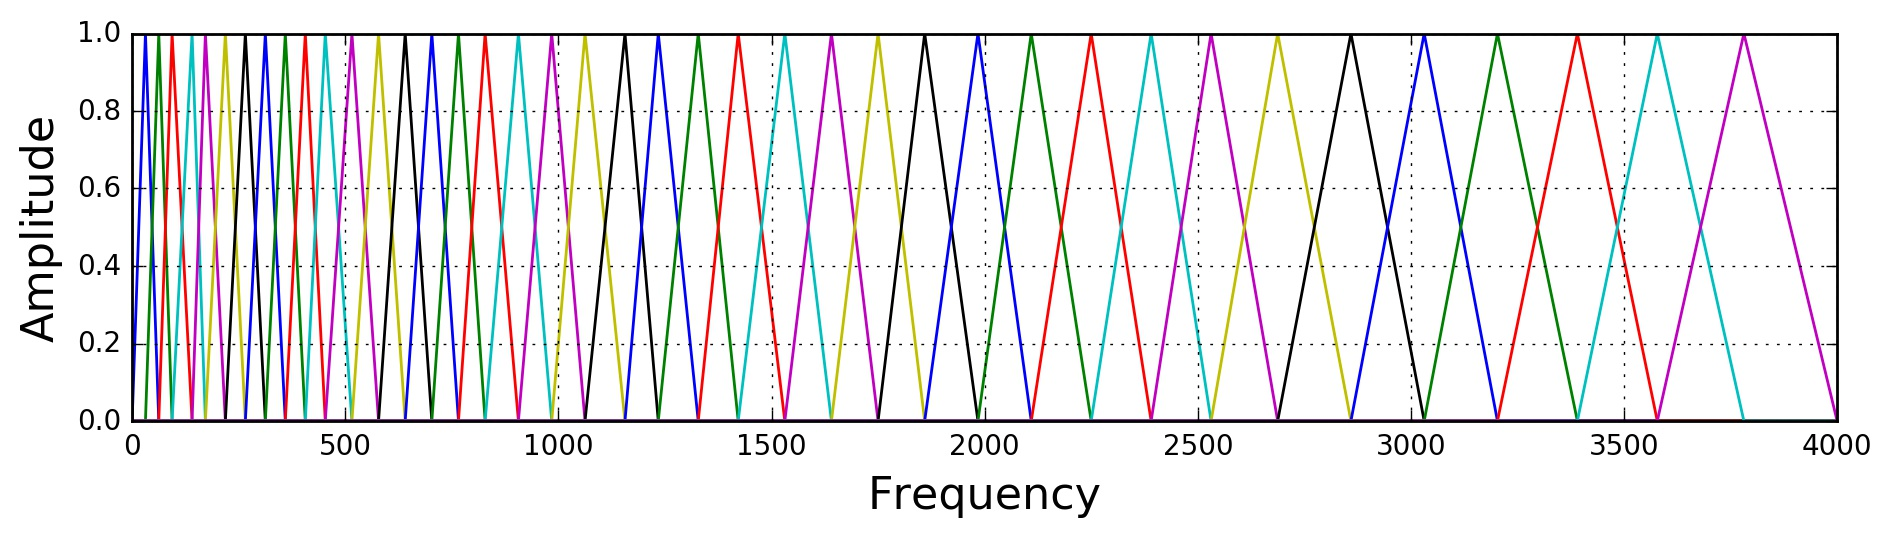
\includegraphics{mel_filters.jpg}
\caption{Mel filter banks}
\end{figure}

Source:
https://haythamfayek.com/2016/04/21/speech-processing-for-machine-learning.html

\hypertarget{log-mel-scale-spectrogram-1}{%
\subsubsection{Log Mel-scale
spectrogram}\label{log-mel-scale-spectrogram-1}}

To convert a spectrogram in linear frequency to a Mel-scale one, for
each frame in the STFT, we weigh the discrete Fourier spectrum by the
Mel filter bank, i.e.~multiply the two values at each frequency.

Further take the log to get the log Mel spectrogram; human ears hear
loudness on a log scale.

\hypertarget{librosa}{%
\subsubsection{librosa}\label{librosa}}

Filter banks: librosa.filters.mel(sr, n\_fft, n\_mels=128, fmin=0.0) Mel
spectrogram: librosa.feature.melspectrogram(y=None, sr=22050,
n\_fft=2048, hop\_length=512). Returns an array of shape = (n\_mels,
n\_frames) (VS spectrogram which returns an array of shape =
(1+n\_fft/2, n\_frames)).

    \hypertarget{mel-filter-banks-visualisation}{%
\subsubsection{Mel filter banks:
visualisation}\label{mel-filter-banks-visualisation}}

    \begin{tcolorbox}[breakable, size=fbox, boxrule=1pt, pad at break*=1mm,colback=cellbackground, colframe=cellborder]
\prompt{In}{incolor}{78}{\boxspacing}
\begin{Verbatim}[commandchars=\\\{\}]
\PY{n}{f\PYZus{}s} \PY{o}{=} \PY{l+m+mi}{16000}
\PY{n}{filterbanks} \PY{o}{=} \PY{n}{librosa}\PY{o}{.}\PY{n}{filters}\PY{o}{.}\PY{n}{mel}\PY{p}{(}\PY{n}{sr}\PY{o}{=}\PY{n}{f\PYZus{}s}\PY{p}{,} \PY{n}{n\PYZus{}fft}\PY{o}{=}\PY{l+m+mi}{512}\PY{p}{,} \PY{n}{n\PYZus{}mels}\PY{o}{=}\PY{l+m+mi}{20}\PY{p}{,} \PY{n}{fmin}\PY{o}{=}\PY{l+m+mf}{0.0}\PY{p}{)}
\end{Verbatim}
\end{tcolorbox}

    \begin{tcolorbox}[breakable, size=fbox, boxrule=1pt, pad at break*=1mm,colback=cellbackground, colframe=cellborder]
\prompt{In}{incolor}{79}{\boxspacing}
\begin{Verbatim}[commandchars=\\\{\}]
\PY{n}{filterbanks}\PY{o}{.}\PY{n}{shape}
\end{Verbatim}
\end{tcolorbox}

            \begin{tcolorbox}[breakable, size=fbox, boxrule=.5pt, pad at break*=1mm, opacityfill=0]
\prompt{Out}{outcolor}{79}{\boxspacing}
\begin{Verbatim}[commandchars=\\\{\}]
(20, 257)
\end{Verbatim}
\end{tcolorbox}
        
    \begin{tcolorbox}[breakable, size=fbox, boxrule=1pt, pad at break*=1mm,colback=cellbackground, colframe=cellborder]
\prompt{In}{incolor}{80}{\boxspacing}
\begin{Verbatim}[commandchars=\\\{\}]
\PY{c+c1}{\PYZsh{} normalise the triangular filters for visualisation}
\PY{n}{filterbanks} \PY{o}{/}\PY{o}{=} \PY{n}{np}\PY{o}{.}\PY{n}{expand\PYZus{}dims}\PY{p}{(}\PY{n}{np}\PY{o}{.}\PY{n}{max}\PY{p}{(}\PY{n}{filterbanks}\PY{p}{,} \PY{n}{axis}\PY{o}{=}\PY{o}{\PYZhy{}}\PY{l+m+mi}{1}\PY{p}{)}\PY{p}{,} \PY{n}{axis}\PY{o}{=}\PY{o}{\PYZhy{}}\PY{l+m+mi}{1}\PY{p}{)}
\end{Verbatim}
\end{tcolorbox}

    \begin{tcolorbox}[breakable, size=fbox, boxrule=1pt, pad at break*=1mm,colback=cellbackground, colframe=cellborder]
\prompt{In}{incolor}{81}{\boxspacing}
\begin{Verbatim}[commandchars=\\\{\}]
\PY{n}{filterbanks\PYZus{}freq} \PY{o}{=} \PY{n}{np}\PY{o}{.}\PY{n}{arange}\PY{p}{(}\PY{n}{filterbanks}\PY{o}{.}\PY{n}{shape}\PY{p}{[}\PY{l+m+mi}{1}\PY{p}{]}\PY{p}{)} \PY{o}{/} \PY{l+m+mi}{512} \PY{o}{*} \PY{n}{f\PYZus{}s}
\end{Verbatim}
\end{tcolorbox}

    \begin{tcolorbox}[breakable, size=fbox, boxrule=1pt, pad at break*=1mm,colback=cellbackground, colframe=cellborder]
\prompt{In}{incolor}{91}{\boxspacing}
\begin{Verbatim}[commandchars=\\\{\}]
\PY{n}{plt}\PY{o}{.}\PY{n}{plot}\PY{p}{(}\PY{n}{filterbanks\PYZus{}freq}\PY{p}{,} \PY{n}{filterbanks}\PY{o}{.}\PY{n}{T}\PY{p}{,} \PY{n}{color}\PY{o}{=}\PY{l+s+s1}{\PYZsq{}}\PY{l+s+s1}{tomato}\PY{l+s+s1}{\PYZsq{}}\PY{p}{)}\PY{p}{;}
\PY{n}{plt}\PY{o}{.}\PY{n}{xlabel}\PY{p}{(}\PY{l+s+s1}{\PYZsq{}}\PY{l+s+s1}{Frequency (Hz)}\PY{l+s+s1}{\PYZsq{}}\PY{p}{)}\PY{p}{;}
\end{Verbatim}
\end{tcolorbox}

    \begin{center}
    \adjustimage{max size={0.9\linewidth}{0.9\paperheight}}{output_60_0.png}
    \end{center}
    { \hspace*{\fill} \\}
    
    \hypertarget{mel-spectrogram}{%
\subsubsection{Mel spectrogram}\label{mel-spectrogram}}

    \begin{tcolorbox}[breakable, size=fbox, boxrule=1pt, pad at break*=1mm,colback=cellbackground, colframe=cellborder]
\prompt{In}{incolor}{103}{\boxspacing}
\begin{Verbatim}[commandchars=\\\{\}]
\PY{c+c1}{\PYZsh{} filename = \PYZsq{}violin\PYZus{}A.wav\PYZsq{}}
\PY{n}{filename} \PY{o}{=} \PY{l+s+s1}{\PYZsq{}}\PY{l+s+s1}{bruckner.wav}\PY{l+s+s1}{\PYZsq{}}
\PY{c+c1}{\PYZsh{} extract sample rate (e.g. 44100Hz) and signal}
\PY{n}{f\PYZus{}s}\PY{p}{,} \PY{n}{x} \PY{o}{=} \PY{n}{wavfile}\PY{o}{.}\PY{n}{read}\PY{p}{(}\PY{n}{filename}\PY{p}{)}
\PY{n}{x} \PY{o}{=} \PY{n}{x} \PY{o}{/} \PY{l+m+mf}{1.0}  \PY{c+c1}{\PYZsh{} convert to float}
\PY{n}{ipyd}\PY{o}{.}\PY{n}{Audio}\PY{p}{(}\PY{n}{rate}\PY{o}{=}\PY{n}{f\PYZus{}s}\PY{p}{,} \PY{n}{data}\PY{o}{=}\PY{n}{x}\PY{p}{)}
\end{Verbatim}
\end{tcolorbox}

            \begin{tcolorbox}[breakable, size=fbox, boxrule=.5pt, pad at break*=1mm, opacityfill=0]
\prompt{Out}{outcolor}{103}{\boxspacing}
\begin{Verbatim}[commandchars=\\\{\}]
<IPython.lib.display.Audio object>
\end{Verbatim}
\end{tcolorbox}
        
    \begin{tcolorbox}[breakable, size=fbox, boxrule=1pt, pad at break*=1mm,colback=cellbackground, colframe=cellborder]
\prompt{In}{incolor}{108}{\boxspacing}
\begin{Verbatim}[commandchars=\\\{\}]
\PY{c+c1}{\PYZsh{} construct Mel spectrogram}
\PY{n}{n\PYZus{}fft} \PY{o}{=} \PY{n+nb}{int}\PY{p}{(}\PY{l+m+mf}{0.025}\PY{o}{*}\PY{n}{f\PYZus{}s}\PY{p}{)}  \PY{c+c1}{\PYZsh{} 25ms}
\PY{n}{hop\PYZus{}length} \PY{o}{=} \PY{n+nb}{int}\PY{p}{(}\PY{l+m+mf}{0.01}\PY{o}{*}\PY{n}{f\PYZus{}s}\PY{p}{)}  \PY{c+c1}{\PYZsh{} 10ms}
\PY{n}{mel\PYZus{}spec} \PY{o}{=} \PY{n}{librosa}\PY{o}{.}\PY{n}{feature}\PY{o}{.}\PY{n}{melspectrogram}\PY{p}{(}\PY{n}{x}\PY{p}{,} \PY{n}{sr}\PY{o}{=}\PY{n}{f\PYZus{}s}\PY{p}{,} \PY{n}{n\PYZus{}fft}\PY{o}{=}\PY{n}{n\PYZus{}fft}\PY{p}{,} \PY{n}{hop\PYZus{}length}\PY{o}{=}\PY{n}{hop\PYZus{}length}\PY{p}{,} \PY{n}{n\PYZus{}mels}\PY{o}{=}\PY{l+m+mi}{128}\PY{p}{)}
\PY{n}{log\PYZus{}mel\PYZus{}spec} \PY{o}{=} \PY{n}{np}\PY{o}{.}\PY{n}{log}\PY{p}{(}\PY{n}{mel\PYZus{}spec}\PY{p}{)}
\end{Verbatim}
\end{tcolorbox}

    \begin{tcolorbox}[breakable, size=fbox, boxrule=1pt, pad at break*=1mm,colback=cellbackground, colframe=cellborder]
\prompt{In}{incolor}{109}{\boxspacing}
\begin{Verbatim}[commandchars=\\\{\}]
\PY{c+c1}{\PYZsh{} shape=(n\PYZus{}mels, n\PYZus{}frames)}
\PY{n}{log\PYZus{}mel\PYZus{}spec}\PY{o}{.}\PY{n}{shape}
\end{Verbatim}
\end{tcolorbox}

            \begin{tcolorbox}[breakable, size=fbox, boxrule=.5pt, pad at break*=1mm, opacityfill=0]
\prompt{Out}{outcolor}{109}{\boxspacing}
\begin{Verbatim}[commandchars=\\\{\}]
(128, 514)
\end{Verbatim}
\end{tcolorbox}
        
    \begin{tcolorbox}[breakable, size=fbox, boxrule=1pt, pad at break*=1mm,colback=cellbackground, colframe=cellborder]
\prompt{In}{incolor}{112}{\boxspacing}
\begin{Verbatim}[commandchars=\\\{\}]
\PY{c+c1}{\PYZsh{} Plot Mel spectrogram}
\PY{n}{fig}\PY{p}{,} \PY{n}{ax} \PY{o}{=} \PY{n}{plt}\PY{o}{.}\PY{n}{subplots}\PY{p}{(}\PY{n}{figsize}\PY{o}{=}\PY{p}{(}\PY{l+m+mi}{9}\PY{p}{,}\PY{l+m+mi}{5}\PY{p}{)}\PY{p}{)}
\PY{n}{img} \PY{o}{=} \PY{n}{librosa}\PY{o}{.}\PY{n}{display}\PY{o}{.}\PY{n}{specshow}\PY{p}{(}\PY{n}{log\PYZus{}mel\PYZus{}spec}\PY{p}{,} \PY{n}{sr}\PY{o}{=}\PY{n}{f\PYZus{}s}\PY{p}{,} 
                        \PY{n}{y\PYZus{}axis}\PY{o}{=}\PY{l+s+s1}{\PYZsq{}}\PY{l+s+s1}{mel}\PY{l+s+s1}{\PYZsq{}}\PY{p}{,} \PY{n}{x\PYZus{}axis}\PY{o}{=}\PY{l+s+s1}{\PYZsq{}}\PY{l+s+s1}{time}\PY{l+s+s1}{\PYZsq{}}\PY{p}{,} \PY{n}{ax}\PY{o}{=}\PY{n}{ax}\PY{p}{,} \PY{n}{fmax}\PY{o}{=}\PY{l+m+mi}{6000}\PY{p}{)}\PY{p}{;}
\PY{n}{plt}\PY{o}{.}\PY{n}{xlabel}\PY{p}{(}\PY{l+s+s1}{\PYZsq{}}\PY{l+s+s1}{Time (s)}\PY{l+s+s1}{\PYZsq{}}\PY{p}{)}\PY{p}{;}
\PY{n}{plt}\PY{o}{.}\PY{n}{ylabel}\PY{p}{(}\PY{l+s+s2}{\PYZdq{}}\PY{l+s+s2}{Frequency (Hz)}\PY{l+s+s2}{\PYZdq{}}\PY{p}{)}\PY{p}{;}
\PY{n}{plt}\PY{o}{.}\PY{n}{ylim}\PY{p}{(}\PY{p}{[}\PY{l+m+mi}{0}\PY{p}{,} \PY{l+m+mi}{1200}\PY{p}{]}\PY{p}{)}
\PY{n}{fig}\PY{o}{.}\PY{n}{colorbar}\PY{p}{(}\PY{n}{img}\PY{p}{,} \PY{n}{ax}\PY{o}{=}\PY{n}{ax}\PY{p}{,} \PY{n+nb}{format}\PY{o}{=}\PY{l+s+s2}{\PYZdq{}}\PY{l+s+si}{\PYZpc{}2.0f}\PY{l+s+s2}{ dB}\PY{l+s+s2}{\PYZdq{}}\PY{p}{)}\PY{p}{;}
\end{Verbatim}
\end{tcolorbox}

    \begin{center}
    \adjustimage{max size={0.9\linewidth}{0.9\paperheight}}{output_65_0.png}
    \end{center}
    { \hspace*{\fill} \\}
    
    \begin{tcolorbox}[breakable, size=fbox, boxrule=1pt, pad at break*=1mm,colback=cellbackground, colframe=cellborder]
\prompt{In}{incolor}{ }{\boxspacing}
\begin{Verbatim}[commandchars=\\\{\}]

\end{Verbatim}
\end{tcolorbox}

    \hypertarget{windowing-pre-emphasis-filter-mel-frequency-cepstral-coefficients-mfcc}{%
\section{4. Windowing, Pre-Emphasis Filter, Mel-Frequency Cepstral Coefficients (MFCC)}\label{windowing-pre-emphasis-filter-mel-frequency-cepstral-coefficients-mfcc}}

\hypertarget{windowing}{%
\subsubsection{Windowing}\label{windowing}}

A \textbf{window function} \(w(t)\) (also known as an apodisation
function or tapering function) is a mathematical function that is
zero-valued outside of some chosen interval, normally symmetric around
the middle of the interval, usually near a maximum in the middle, and
usually tapering away from the middle.

In signal processing, we weigh a signal \(x_n\) by the discretisation of
a window function \(w_n\), i.e.~we compute the point-wise product

\[\tilde{x}_n\equiv x_n \cdot w_n. \tag{8}\]

The discrete Fourier transform \(X_k\) defined in (1) in Section 1
should instead be understood as that of \(\tilde{x}_n\).

A benefit of using such a window function is that it reduces the
boundary effect of the signal (or a frame thereof in STFT), rendering
the resulting DFT smoother.

A popular choice of the window function is the \textbf{Hamming
function}, which is a special case of a \textbf{cosine-sum window
function} (see Wikipedia).

\hypertarget{pre-emphasis-filter}{%
\subsubsection{Pre-emphasis filter}\label{pre-emphasis-filter}}

The \textbf{pre-emphasis} \(y_n\) of a signal \(x_n\) is defined as

\[ y_n \equiv x_n - \alpha x_{n-1},\tag{9}\]

where typically the coefficient takes the value \(\alpha=0.97\).

A \textbf{pre-emphasis filter} is a noise reduction technique in which a
signal's weaker, higher frequencies are boosted before they are
transmitted or recorded onto a storage medium. Upon playback, a
\textbf{de-emphasis filter} is applied to reverse the process. The
result is a higher signal-to-noise ratio; the original frequencies are
restored, but noise that was introduced by the storage medium,
transmission equipment, or analog/digital conversions is quieter than it
would have been if no filtering had been done. Pre- and de-emphasis can
be collectively referred to as just \textbf{emphasis}.

Source: https://wiki.hydrogenaud.io/index.php?title=Pre-emphasis

The pre-emphasis operation is applied, where applicable, on the signal
as the 0-th step, i.e.~before weighing it by the window function.

\hypertarget{mel-frequency-cepstral-coefficients-mfcc}{%
\subsubsection{Mel-Frequency Cepstral Coefficients
(MFCC)}\label{mel-frequency-cepstral-coefficients-mfcc}}

In obtaining the (log) Mel spectrogram, we used a filter bank which
contains overlapping triangular filters. Because of the overlapping, the
filter bank energies (represented by the spectrogram) are quite
correlated with each other. The \textbf{discrete cosine transform (DCT)}
decorrelates the energies, which means that the diagonal covariance
matrices can be used to model the features. The resulting DCT
coefficients are called the \textbf{Mel-frequency cepstral coefficients
(MFCC)} (compare with the definition of cepstral coefficients in
Wikipedia).

The higher DCT coefficients, which represent fast changes in the filter
bank energies, degrade performance in \textbf{Automatic Speech
Recognition (ASR)}. Thus, one typically discards them and \textbf{retain
only the cepstral coefficients 2-13} to get a small improvement.

References:
https://haythamfayek.com/2016/04/21/speech-processing-for-machine-learning.html
http://practicalcryptography.com/miscellaneous/machine-learning/guide-mel-frequency-cepstral-coefficients-mfccs/

\hypertarget{librosa}{%
\subsubsection{librosa}\label{librosa}}

MFCC: librosa.feature.mfcc(y=None, sr=22050, n\_mfcc=20)

    \hypertarget{pre-emphasis}{%
\subsubsection{Pre-Emphasis}\label{pre-emphasis}}

    \begin{tcolorbox}[breakable, size=fbox, boxrule=1pt, pad at break*=1mm,colback=cellbackground, colframe=cellborder]
\prompt{In}{incolor}{121}{\boxspacing}
\begin{Verbatim}[commandchars=\\\{\}]
\PY{k}{def} \PY{n+nf}{preemphasis}\PY{p}{(}\PY{n}{x}\PY{p}{,} \PY{n}{alpha}\PY{o}{=}\PY{l+m+mf}{0.97}\PY{p}{)}\PY{p}{:}
    \PY{k}{return} \PY{n}{np}\PY{o}{.}\PY{n}{append}\PY{p}{(}\PY{n}{x}\PY{p}{[}\PY{l+m+mi}{0}\PY{p}{]}\PY{p}{,} \PY{n}{x}\PY{p}{[}\PY{l+m+mi}{1}\PY{p}{:}\PY{p}{]} \PY{o}{\PYZhy{}} \PY{n}{alpha} \PY{o}{*} \PY{n}{x}\PY{p}{[}\PY{p}{:}\PY{o}{\PYZhy{}}\PY{l+m+mi}{1}\PY{p}{]}\PY{p}{)}
\end{Verbatim}
\end{tcolorbox}

    \begin{tcolorbox}[breakable, size=fbox, boxrule=1pt, pad at break*=1mm,colback=cellbackground, colframe=cellborder]
\prompt{In}{incolor}{113}{\boxspacing}
\begin{Verbatim}[commandchars=\\\{\}]
\PY{n}{filename} \PY{o}{=} \PY{l+s+s1}{\PYZsq{}}\PY{l+s+s1}{violin\PYZus{}A.wav}\PY{l+s+s1}{\PYZsq{}}
\PY{c+c1}{\PYZsh{} filename = \PYZsq{}bruckner.wav\PYZsq{}}
\PY{c+c1}{\PYZsh{} extract sample rate (e.g. 44100Hz) and signal}
\PY{n}{f\PYZus{}s}\PY{p}{,} \PY{n}{x} \PY{o}{=} \PY{n}{wavfile}\PY{o}{.}\PY{n}{read}\PY{p}{(}\PY{n}{filename}\PY{p}{)}
\PY{n}{x} \PY{o}{=} \PY{n}{x} \PY{o}{/} \PY{l+m+mf}{1.0}  \PY{c+c1}{\PYZsh{} convert to float}
\PY{n}{ipyd}\PY{o}{.}\PY{n}{Audio}\PY{p}{(}\PY{n}{rate}\PY{o}{=}\PY{n}{f\PYZus{}s}\PY{p}{,} \PY{n}{data}\PY{o}{=}\PY{n}{x}\PY{p}{)}
\end{Verbatim}
\end{tcolorbox}

            \begin{tcolorbox}[breakable, size=fbox, boxrule=.5pt, pad at break*=1mm, opacityfill=0]
\prompt{Out}{outcolor}{113}{\boxspacing}
\begin{Verbatim}[commandchars=\\\{\}]
<IPython.lib.display.Audio object>
\end{Verbatim}
\end{tcolorbox}
        
    \begin{tcolorbox}[breakable, size=fbox, boxrule=1pt, pad at break*=1mm,colback=cellbackground, colframe=cellborder]
\prompt{In}{incolor}{137}{\boxspacing}
\begin{Verbatim}[commandchars=\\\{\}]
\PY{n}{N} \PY{o}{=} \PY{n+nb}{len}\PY{p}{(}\PY{n}{x}\PY{p}{)}
\PY{n}{w} \PY{o}{=} \PY{n}{np}\PY{o}{.}\PY{n}{hamming}\PY{p}{(}\PY{n}{N}\PY{p}{)}
\PY{c+c1}{\PYZsh{} FFT}
\PY{n}{X} \PY{o}{=} \PY{n}{np}\PY{o}{.}\PY{n}{fft}\PY{o}{.}\PY{n}{fft}\PY{p}{(}\PY{n}{x}\PY{o}{*}\PY{n}{w}\PY{p}{)}

\PY{c+c1}{\PYZsh{} log plot of DFT without pre\PYZhy{}emphasis}
\PY{n}{plt}\PY{o}{.}\PY{n}{figure}\PY{p}{(}\PY{n}{figsize}\PY{o}{=}\PY{p}{(}\PY{l+m+mi}{10}\PY{p}{,}\PY{l+m+mi}{6}\PY{p}{)}\PY{p}{)}
\PY{n}{plt}\PY{o}{.}\PY{n}{plot}\PY{p}{(}\PY{n}{np}\PY{o}{.}\PY{n}{linspace}\PY{p}{(}\PY{l+m+mi}{0}\PY{p}{,} \PY{n}{f\PYZus{}s}\PY{o}{*}\PY{p}{(}\PY{n}{N}\PY{o}{\PYZhy{}}\PY{l+m+mi}{1}\PY{p}{)}\PY{o}{/}\PY{n}{N}\PY{p}{,} \PY{n}{N}\PY{p}{)}\PY{p}{,} \PY{n}{np}\PY{o}{.}\PY{n}{log}\PY{p}{(}\PY{n}{np}\PY{o}{.}\PY{n}{abs}\PY{p}{(}\PY{n}{X}\PY{p}{)}\PY{p}{)}\PY{p}{,} \PY{n}{color}\PY{o}{=}\PY{l+s+s1}{\PYZsq{}}\PY{l+s+s1}{blue}\PY{l+s+s1}{\PYZsq{}}\PY{p}{,} \PY{n}{alpha}\PY{o}{=}\PY{l+m+mf}{0.5}\PY{p}{)}
\PY{n}{plt}\PY{o}{.}\PY{n}{xlabel}\PY{p}{(}\PY{l+s+s1}{\PYZsq{}}\PY{l+s+s1}{Frequency (Hz)}\PY{l+s+s1}{\PYZsq{}}\PY{p}{)}
\PY{n}{plt}\PY{o}{.}\PY{n}{ylabel}\PY{p}{(}\PY{l+s+s2}{\PYZdq{}}\PY{l+s+s2}{Amplitude (log)}\PY{l+s+s2}{\PYZdq{}}\PY{p}{)}

\PY{c+c1}{\PYZsh{} pre\PYZhy{}emphasis}
\PY{n}{x\PYZus{}preem} \PY{o}{=} \PY{n}{preemphasis}\PY{p}{(}\PY{n}{x}\PY{p}{)}
\PY{c+c1}{\PYZsh{} FFT}
\PY{n}{X\PYZus{}preem} \PY{o}{=} \PY{n}{np}\PY{o}{.}\PY{n}{fft}\PY{o}{.}\PY{n}{fft}\PY{p}{(}\PY{n}{x\PYZus{}preem}\PY{o}{*}\PY{n}{w}\PY{p}{)}

\PY{c+c1}{\PYZsh{} log plot of DFT WITH pre\PYZhy{}emphasis}
\PY{n}{plt}\PY{o}{.}\PY{n}{plot}\PY{p}{(}\PY{n}{np}\PY{o}{.}\PY{n}{linspace}\PY{p}{(}\PY{l+m+mi}{0}\PY{p}{,} \PY{n}{f\PYZus{}s}\PY{o}{*}\PY{p}{(}\PY{n}{N}\PY{o}{\PYZhy{}}\PY{l+m+mi}{1}\PY{p}{)}\PY{o}{/}\PY{n}{N}\PY{p}{,} \PY{n}{N}\PY{p}{)}\PY{p}{,} \PY{n}{np}\PY{o}{.}\PY{n}{log}\PY{p}{(}\PY{n}{np}\PY{o}{.}\PY{n}{abs}\PY{p}{(}\PY{n}{X\PYZus{}preem}\PY{p}{)}\PY{p}{)}\PY{p}{,} \PY{n}{color}\PY{o}{=}\PY{l+s+s1}{\PYZsq{}}\PY{l+s+s1}{red}\PY{l+s+s1}{\PYZsq{}}\PY{p}{,} \PY{n}{alpha}\PY{o}{=}\PY{l+m+mf}{0.5}\PY{p}{)}
\PY{n}{plt}\PY{o}{.}\PY{n}{xlabel}\PY{p}{(}\PY{l+s+s1}{\PYZsq{}}\PY{l+s+s1}{Frequency (Hz)}\PY{l+s+s1}{\PYZsq{}}\PY{p}{)}
\PY{n}{plt}\PY{o}{.}\PY{n}{ylabel}\PY{p}{(}\PY{l+s+s2}{\PYZdq{}}\PY{l+s+s2}{Amplitude (log)}\PY{l+s+s2}{\PYZdq{}}\PY{p}{)}
\PY{n}{plt}\PY{o}{.}\PY{n}{xlim}\PY{p}{(}\PY{p}{[}\PY{l+m+mi}{5000}\PY{p}{,} \PY{l+m+mi}{22050}\PY{p}{]}\PY{p}{)}\PY{p}{;}
\PY{n}{plt}\PY{o}{.}\PY{n}{ylim}\PY{p}{(}\PY{p}{[}\PY{l+m+mf}{2.5}\PY{p}{,} \PY{l+m+mf}{15.}\PY{p}{]}\PY{p}{)}\PY{p}{;}
\end{Verbatim}
\end{tcolorbox}

    \begin{center}
    \adjustimage{max size={0.9\linewidth}{0.9\paperheight}}{output_71_0.png}
    \end{center}
    { \hspace*{\fill} \\}
    
    Indeed, high frequency modes are boosted.

    \hypertarget{mfccs}{%
\subsubsection{MFCCs}\label{mfccs}}

    \begin{tcolorbox}[breakable, size=fbox, boxrule=1pt, pad at break*=1mm,colback=cellbackground, colframe=cellborder]
\prompt{In}{incolor}{147}{\boxspacing}
\begin{Verbatim}[commandchars=\\\{\}]
\PY{c+c1}{\PYZsh{} filename = \PYZsq{}violin\PYZus{}A.wav\PYZsq{}}
\PY{n}{filename} \PY{o}{=} \PY{l+s+s1}{\PYZsq{}}\PY{l+s+s1}{bruckner.wav}\PY{l+s+s1}{\PYZsq{}}
\PY{c+c1}{\PYZsh{} extract sample rate (e.g. 44100Hz) and signal}
\PY{n}{f\PYZus{}s}\PY{p}{,} \PY{n}{x} \PY{o}{=} \PY{n}{wavfile}\PY{o}{.}\PY{n}{read}\PY{p}{(}\PY{n}{filename}\PY{p}{)}
\PY{n}{x} \PY{o}{=} \PY{n}{x} \PY{o}{/} \PY{l+m+mf}{1.0}  \PY{c+c1}{\PYZsh{} convert to float}
\PY{n}{ipyd}\PY{o}{.}\PY{n}{Audio}\PY{p}{(}\PY{n}{rate}\PY{o}{=}\PY{n}{f\PYZus{}s}\PY{p}{,} \PY{n}{data}\PY{o}{=}\PY{n}{x}\PY{p}{)}
\end{Verbatim}
\end{tcolorbox}

            \begin{tcolorbox}[breakable, size=fbox, boxrule=.5pt, pad at break*=1mm, opacityfill=0]
\prompt{Out}{outcolor}{147}{\boxspacing}
\begin{Verbatim}[commandchars=\\\{\}]
<IPython.lib.display.Audio object>
\end{Verbatim}
\end{tcolorbox}
        
    \begin{tcolorbox}[breakable, size=fbox, boxrule=1pt, pad at break*=1mm,colback=cellbackground, colframe=cellborder]
\prompt{In}{incolor}{151}{\boxspacing}
\begin{Verbatim}[commandchars=\\\{\}]
\PY{c+c1}{\PYZsh{} construct MFCCs}
\PY{n}{n\PYZus{}fft} \PY{o}{=} \PY{n+nb}{int}\PY{p}{(}\PY{l+m+mf}{0.025}\PY{o}{*}\PY{n}{f\PYZus{}s}\PY{p}{)}  \PY{c+c1}{\PYZsh{} 25ms}
\PY{n}{hop\PYZus{}length} \PY{o}{=} \PY{n+nb}{int}\PY{p}{(}\PY{l+m+mf}{0.01}\PY{o}{*}\PY{n}{f\PYZus{}s}\PY{p}{)}  \PY{c+c1}{\PYZsh{} 10ms}

\PY{n}{mfcc} \PY{o}{=} \PY{n}{librosa}\PY{o}{.}\PY{n}{feature}\PY{o}{.}\PY{n}{mfcc}\PY{p}{(}\PY{n}{x}\PY{p}{,} \PY{n}{sr}\PY{o}{=}\PY{n}{f\PYZus{}s}\PY{p}{,} \PY{n}{n\PYZus{}mfcc}\PY{o}{=}\PY{l+m+mi}{13}\PY{p}{,} \PY{n}{n\PYZus{}mels}\PY{o}{=}\PY{l+m+mi}{24}\PY{p}{,} 
                            \PY{n}{n\PYZus{}fft}\PY{o}{=}\PY{n}{n\PYZus{}fft}\PY{p}{,} \PY{n}{hop\PYZus{}length}\PY{o}{=}\PY{n}{hop\PYZus{}length}\PY{p}{,} 
                            \PY{n}{fmin}\PY{o}{=}\PY{l+m+mi}{64}\PY{p}{,} \PY{n}{fmax}\PY{o}{=}\PY{l+m+mi}{8000}\PY{p}{)}

\PY{n}{librosa}\PY{o}{.}\PY{n}{display}\PY{o}{.}\PY{n}{specshow}\PY{p}{(}\PY{n}{mfcc}\PY{p}{,} \PY{n}{x\PYZus{}axis}\PY{o}{=}\PY{l+s+s1}{\PYZsq{}}\PY{l+s+s1}{time}\PY{l+s+s1}{\PYZsq{}}\PY{p}{)}\PY{p}{;}
\PY{n}{plt}\PY{o}{.}\PY{n}{xlabel}\PY{p}{(}\PY{l+s+s1}{\PYZsq{}}\PY{l+s+s1}{Time (s)}\PY{l+s+s1}{\PYZsq{}}\PY{p}{)}\PY{p}{;}
\end{Verbatim}
\end{tcolorbox}

    \begin{center}
    \adjustimage{max size={0.9\linewidth}{0.9\paperheight}}{output_75_0.png}
    \end{center}
    { \hspace*{\fill} \\}
    
    \begin{tcolorbox}[breakable, size=fbox, boxrule=1pt, pad at break*=1mm,colback=cellbackground, colframe=cellborder]
\prompt{In}{incolor}{ }{\boxspacing}
\begin{Verbatim}[commandchars=\\\{\}]

\end{Verbatim}
\end{tcolorbox}

    \begin{tcolorbox}[breakable, size=fbox, boxrule=1pt, pad at break*=1mm,colback=cellbackground, colframe=cellborder]
\prompt{In}{incolor}{ }{\boxspacing}
\begin{Verbatim}[commandchars=\\\{\}]

\end{Verbatim}
\end{tcolorbox}

    \hypertarget{summary-from-signal-to-mel-frequency-cepstral-coefficients-mfcc}{%
\subsection{5. Summary: From Signal to Mel-Frequency Cepstral
Coefficients
(MFCC)}\label{summary-from-signal-to-mel-frequency-cepstral-coefficients-mfcc}}

The general workflow of obtaining a Mel-frequency cepstral coefficients
(MFCC) from a signal is as follows.

\begin{enumerate}
\def\labelenumi{\arabic{enumi}.}
\setcounter{enumi}{-1}
\tightlist
\item
  Apply a \textbf{pre-emphasis filter}, where applicable, to boost
  high-frequency signals.
\item
  Apply a \textbf{window function} to smooth out boundary effects, and
  compute the \textbf{short-time Fourier transform (STFT)}. The
  resulting discrete Fourier coefficients are \emph{complex} numbers.
\item
  Take the \textbf{absolute values} of the Fourier coefficients to get
  the power spectrum.
\item
  Apply a \textbf{Mel filter bank} and take the \textbf{log scale} to
  reflect how human ears perceive sound. The result is a \textbf{log
  Mel-scale spectrogram}. \textbf{MFCC:}
\item
  Apply a \textbf{discrete cosin transform (DCT)} to de-correlate filter
  bank energies that result from overlapping triangular Mel filters. The
  DCT coefficients are called the \textbf{Mel-frequency cepstral
  coefficients (MFCC)}.
\item
  Keep only the 2-13 \textbf{MFCCs} for Automatic Speech Recognition
  (ASR), because the higher MFCCs represent fast changes in the filter
  bank energies, which degrade performance.
\end{enumerate}

    \begin{tcolorbox}[breakable, size=fbox, boxrule=1pt, pad at break*=1mm,colback=cellbackground, colframe=cellborder]
\prompt{In}{incolor}{ }{\boxspacing}
\begin{Verbatim}[commandchars=\\\{\}]

\end{Verbatim}
\end{tcolorbox}

    \begin{tcolorbox}[breakable, size=fbox, boxrule=1pt, pad at break*=1mm,colback=cellbackground, colframe=cellborder]
\prompt{In}{incolor}{ }{\boxspacing}
\begin{Verbatim}[commandchars=\\\{\}]

\end{Verbatim}
\end{tcolorbox}

    \begin{tcolorbox}[breakable, size=fbox, boxrule=1pt, pad at break*=1mm,colback=cellbackground, colframe=cellborder]
\prompt{In}{incolor}{ }{\boxspacing}
\begin{Verbatim}[commandchars=\\\{\}]

\end{Verbatim}
\end{tcolorbox}

    \begin{tcolorbox}[breakable, size=fbox, boxrule=1pt, pad at break*=1mm,colback=cellbackground, colframe=cellborder]
\prompt{In}{incolor}{ }{\boxspacing}
\begin{Verbatim}[commandchars=\\\{\}]

\end{Verbatim}
\end{tcolorbox}

    \begin{tcolorbox}[breakable, size=fbox, boxrule=1pt, pad at break*=1mm,colback=cellbackground, colframe=cellborder]
\prompt{In}{incolor}{ }{\boxspacing}
\begin{Verbatim}[commandchars=\\\{\}]

\end{Verbatim}
\end{tcolorbox}

    \begin{tcolorbox}[breakable, size=fbox, boxrule=1pt, pad at break*=1mm,colback=cellbackground, colframe=cellborder]
\prompt{In}{incolor}{ }{\boxspacing}
\begin{Verbatim}[commandchars=\\\{\}]

\end{Verbatim}
\end{tcolorbox}

    \begin{tcolorbox}[breakable, size=fbox, boxrule=1pt, pad at break*=1mm,colback=cellbackground, colframe=cellborder]
\prompt{In}{incolor}{ }{\boxspacing}
\begin{Verbatim}[commandchars=\\\{\}]

\end{Verbatim}
\end{tcolorbox}

    \begin{tcolorbox}[breakable, size=fbox, boxrule=1pt, pad at break*=1mm,colback=cellbackground, colframe=cellborder]
\prompt{In}{incolor}{ }{\boxspacing}
\begin{Verbatim}[commandchars=\\\{\}]

\end{Verbatim}
\end{tcolorbox}

    \begin{tcolorbox}[breakable, size=fbox, boxrule=1pt, pad at break*=1mm,colback=cellbackground, colframe=cellborder]
\prompt{In}{incolor}{ }{\boxspacing}
\begin{Verbatim}[commandchars=\\\{\}]

\end{Verbatim}
\end{tcolorbox}

    \begin{tcolorbox}[breakable, size=fbox, boxrule=1pt, pad at break*=1mm,colback=cellbackground, colframe=cellborder]
\prompt{In}{incolor}{ }{\boxspacing}
\begin{Verbatim}[commandchars=\\\{\}]

\end{Verbatim}
\end{tcolorbox}


    % Add a bibliography block to the postdoc
    
    
    
\end{document}
